\section{Data Analysis of Study}
As discussed, the participants had to fill out a small questionnaire every day in the evening and these answers were then matched against the computed results. The study resulted in a dataset with 205 days of data, corresponding to 2.51M timestamped location data points, spread over 10 participants. Table \ref{tab:location-samples} shows the overview of the data collected for each participant, including the number of points, number of days and the storage requirements for the collected data.
\begin{table}[]
    \centering
        \begin{tabular}{|l|l|l|l|l|l|}
        \hline
        {\ul \textbf{P}} & {\ul \textbf{Days}} & {\ul \textbf{Samples}} & {\ul \textbf{MB}} & {\ul \textbf{Samples/day}} & {\ul \textbf{MB/day}} \\ \hline
        \textbf{P1}                & 23                   & 181                        & 17.3                           & 7878.8                              & 0.8                              \\ \hline
        \textbf{P2}                & 25                   & 142                        & 13.6                           & 5684.4                              & 0.5                             \\ \hline
        \textbf{P3}                & 21                   & 101                        & 9.7                            & 4850.7                              & 0.5                             \\ \hline
        \textbf{P4}                & 22                   & 98                         & 9.4                            & 4494.9                              & 0.4                             \\ \hline
        \textbf{P5}                & 14                   & 209                        & 20.0                           & 14977.4                             & 1.4                             \\ \hline
        \textbf{P6}                & 26                   & 101                        & 9.7                            & 3922.8                              & 0.4                             \\ \hline
        \textbf{P7}                & 23                   & 111                       & 106.4                          & 48525.0                             & 4.6                             \\ \hline
        \textbf{P8}                & 15                   & 141                        & 13.5                           & 9417.3                              & 0.9                              \\ \hline
        \textbf{P9}                & 12                   & 51                         & 4.9                            & 4311.7                              & 0.4                              \\ \hline
        \textbf{R}                 & 24                   & 365                        & 34.9                           & 15233.6                             & 1.5                                    \\ \hline
        \end{tabular}

    \caption{The overview of collected Location Samples for each participant in the study}
    \label{tab:location-samples}
\end{table}

The answers were of a different format than the computed features and therefore had to be converted into scalars such that they could be compared directly to the  features. For the Home Stay feature, the answer the users gave was the number of hours away from home, at the time of registering. It was assumed that most people be registering at home, since the diary was filled out in the evening. Therefore for calculating the Home Stay value from a given answer $a$, equation \ref{eq:home-stay-ans} was applied:

\begin{equation}
\label{eq:home-stay-ans}
    h = \frac{t - a }{t}
\end{equation}

Here, $t$ refers to the timestamp at which the diary was filled out.

For the \textit{Routine Index}, the answer (a number of 0 to 5) was transformed to scalar between 0 and 1, i.e. let the scale value be $s \in \{0, 1, 2, 3, 4, 5\}$, then the corresponding \textit{Routine Index} is calculated using equation \ref{eq:routine-ans}.

\begin{equation}
\label{eq:routine-ans}
    r = \frac{s}{s_{max}}, \quad s_{max} = 5
\end{equation}

Regarding data collection, figure \ref{fig:plot-num-points-stops} displays how much data was collected per participant. From this figure it is clear that some participants did not collect nearly as much data as others, and because of this their computed features are expected to be more inaccurate. It was also discovered that the number of stops found is not necessarily correlated with the number of location samples found, as can be seen for participant P7. This can be due to reasons such as moving around much less, which results in fewer, but Stops with a longer duration being found. 

\begin{figure}
    \centering
    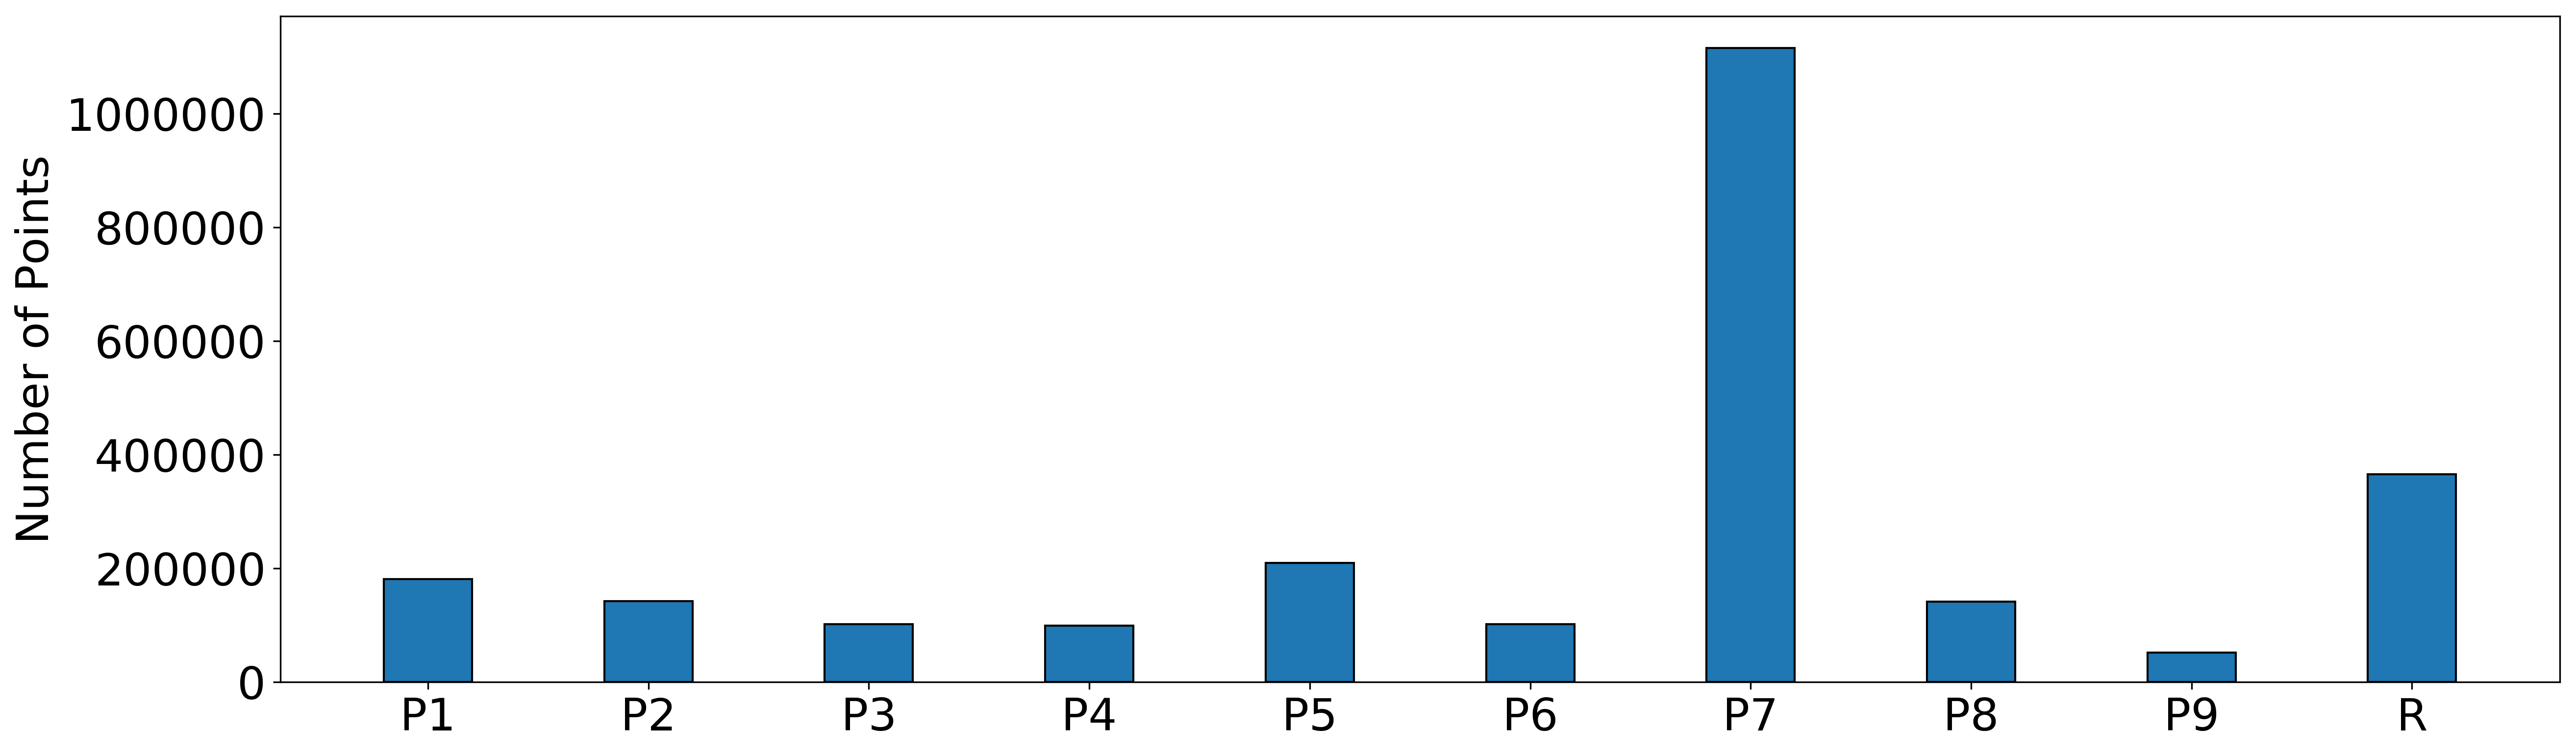
\includegraphics[width=\textwidth]{images/study/storage/num_points.png}
    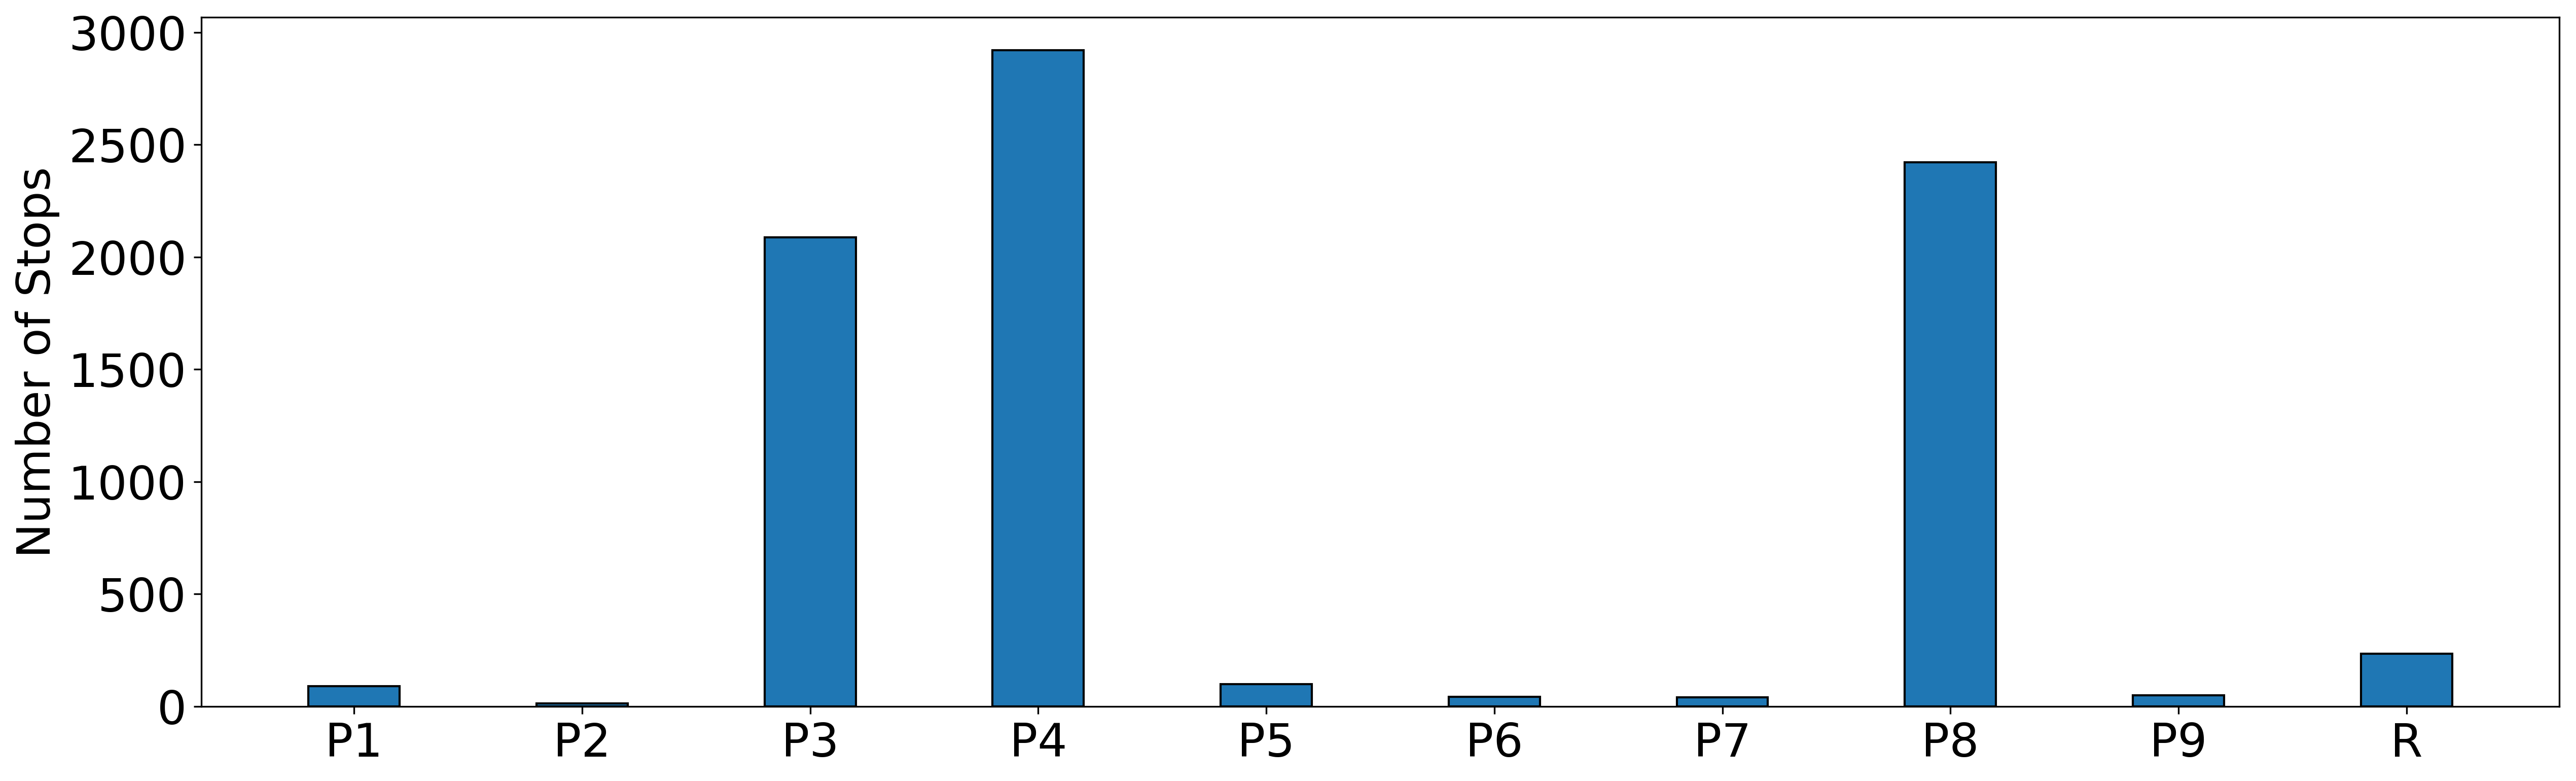
\includegraphics[width=\textwidth]{images/study/storage/num_stops.png}
    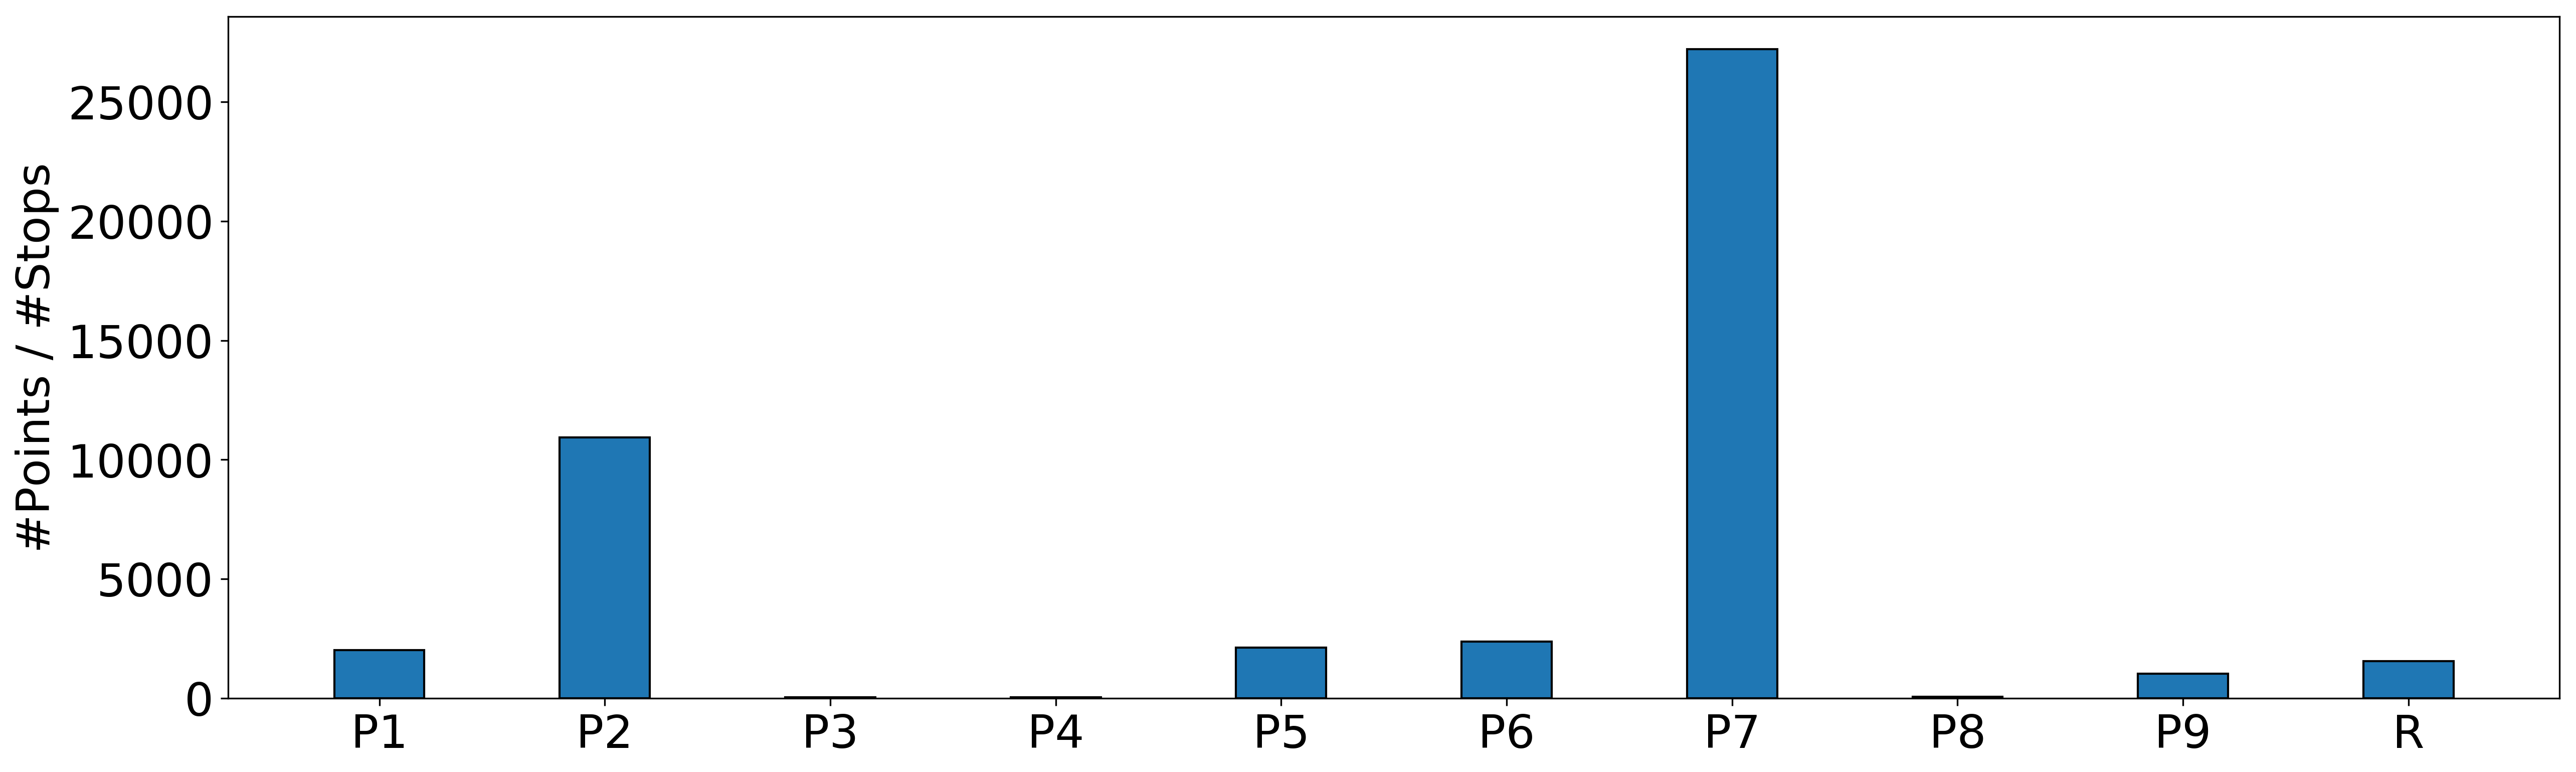
\includegraphics[width=\textwidth]{images/study/storage/compression_N.png}
    \caption{The number of raw Location Samples (top) and the number of Stops (middle) collected, and the ratio between the two, for each participant}
    \label{fig:plot-num-points-stops}
\end{figure}

\begin{figure}
    \centering
    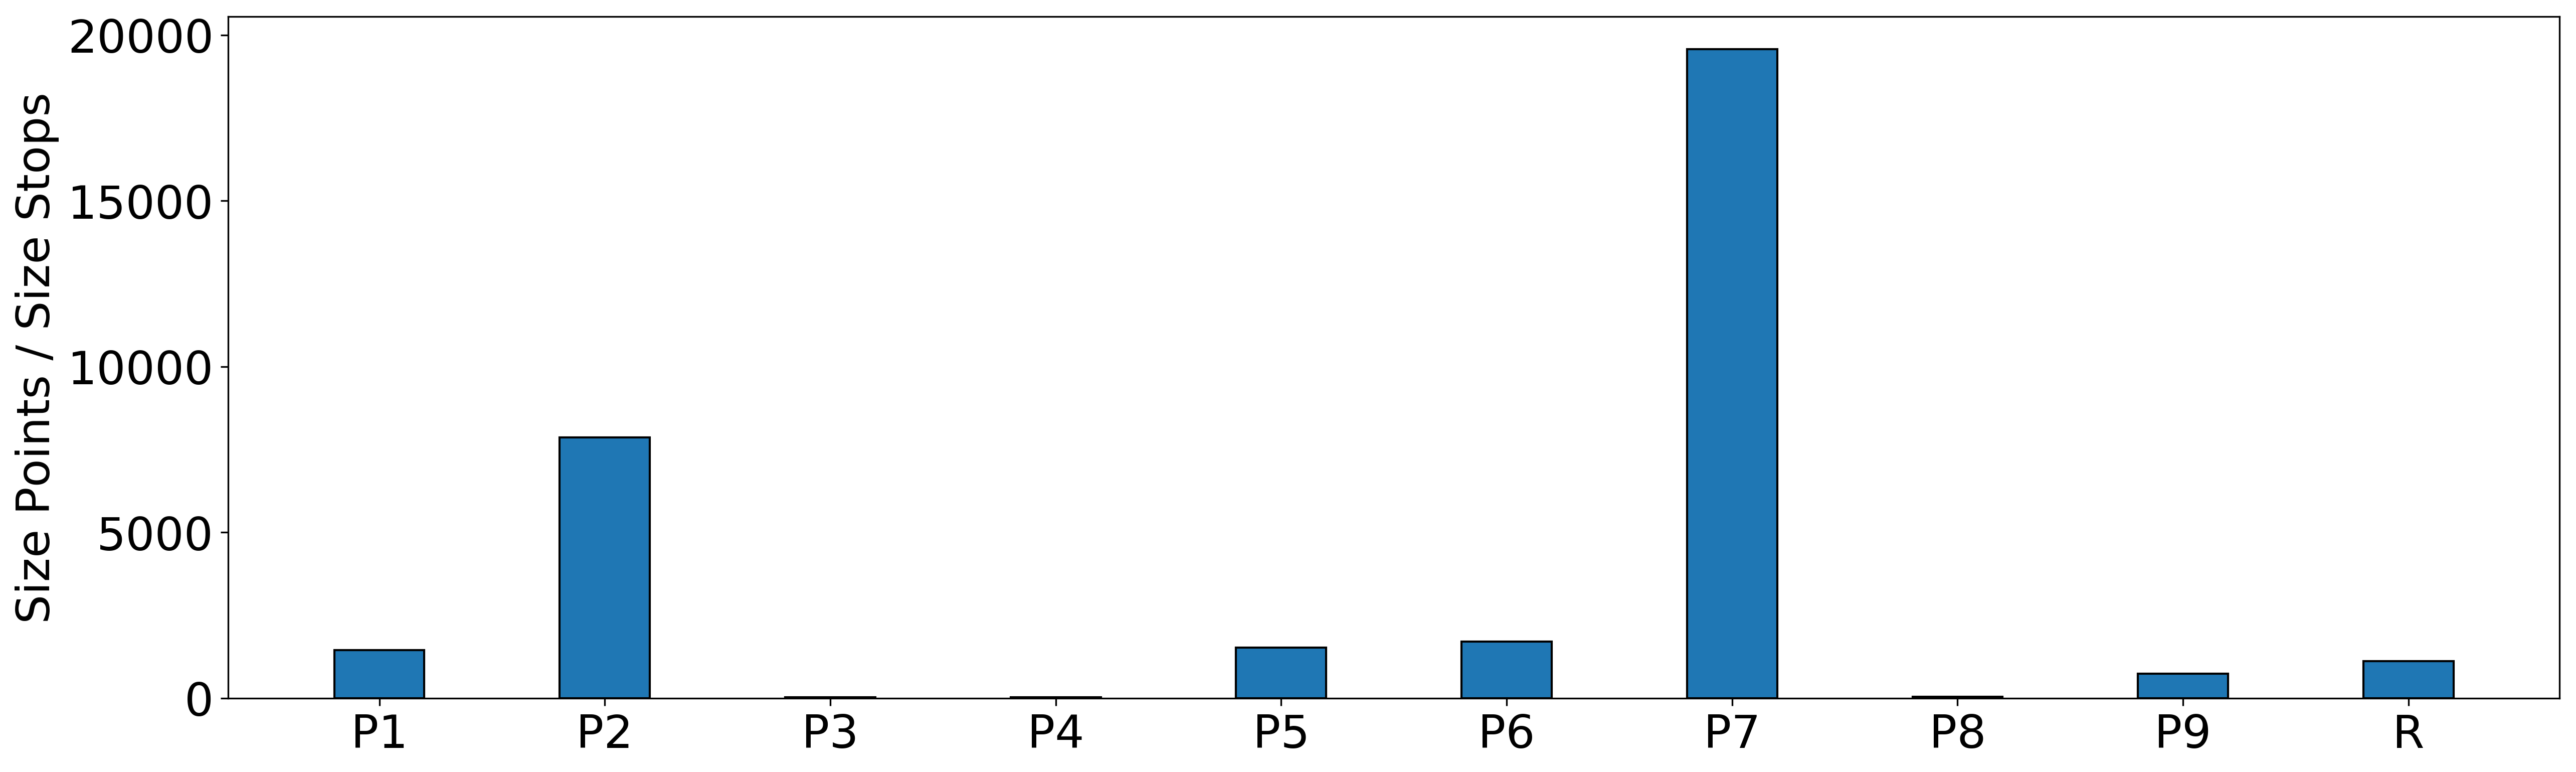
\includegraphics[width=\textwidth]{images/study/storage/compression_mb.png}
    \caption{The ratio between Location Samples and Stops expressed in terms of storage, in MB}
    \label{fig:plot-num-points-stops}
\end{figure}

It was computed based on file size, the average size of a serialized \textit{LocationSample} is 100 bytes, and a \textit{Stop} is 139 bytes. With this information it is possible to calculate the compression rate for each participant, i.e. how much their dataset was reduced by converting Location Samples into Stops, and this is shown in Figure \ref{fig:plot-num-points-stops}. 



The number of valid days for a specific feature is a day for which the user gave answers, and the feature could be calculated. If the user for example turned off their phone during the night, the home stay feature could not be calculated, but the routine index feature and the number of places will likely still have been calculated.


\subsection{Subjectivity of Answers and Ground Truth}
A thing to keep in mind is that the participants' answers are not ground truth, and there are multiple reasons why a participants answer may be inaccurate. Firstly, people's subjective recollection is not necessarily as accurate as they think it might me. Secondly, it was not communicated explicitly to the participants what exactly counts as a place, and how their 'routine' is calculated - this means that participants may have filled out the questionnaire differently, given the same ground truth data - for example whether or not being in the garden counts as being home. Secondly, some users misunderstood the routine scale and users whose data looked strange were contacted afterwards to enquire about whether they had misunderstood the question and if so the answers were corrected as much as could be done. Lastly, the hour away from home and routine index answers were very course grained, and therefore the participants were probably rarely able to give exact answers, according to the their own recollection. 

\subsection{Missing Data and Correcting Data}
Some users missed several days of filling out the diary which meant the computed features for that day could not be compared to a subjective measurement. Figure \ref{fig:plot-days-answered} shows the number of total days where a participant participated in the study where data was collected vs the days on which they provided an answer. For data analysis it was only possible to calculate the error between computed features and the answers given if the participant actually gave an answer. This mean that for some participants, a lot of data was unfortunately not usable for the data analysis. As an example, it was considered whether or not to entirely get rid of P9 since he or she has very little data both terms of total days collected and even fewer in terms of days with answers. 

\begin{figure}
    \centering
    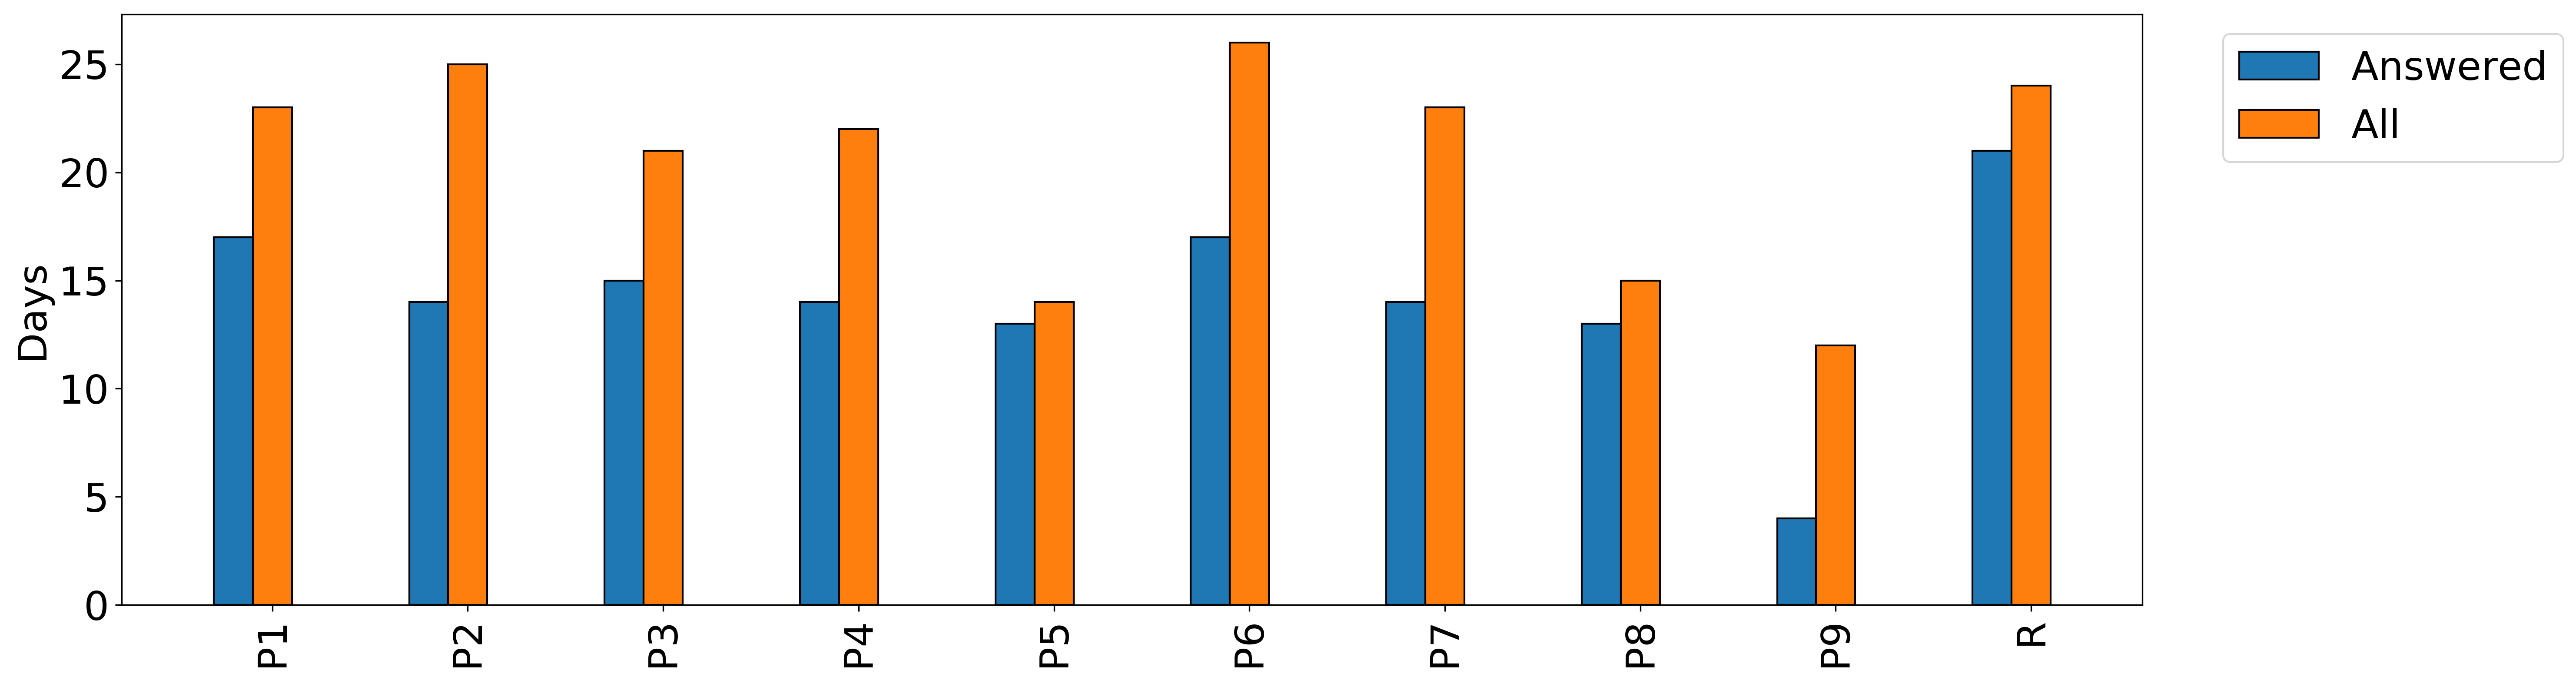
\includegraphics[width=\textwidth]{images/study/storage/answers_days_plot.png}
    \caption{The total number of days of participation vs the days for which the diary was filled out by the participant. As can be seen, some users often forgot to give an answer}
    \label{fig:plot-days-answered}
\end{figure}

Another problem which was encountered was when participants would fill out the questionnaire for day $n$ during the night, which mean the resulting date was $n+1$, i.e. the wrong date. This was simple enough to fix by simply moving all answers given between 00:00 and 10:00 to the previous date which got rid of all the problematic data points. In addition some users entirely forgot certain days but remembered it the following day, and reported it manually to the researcher, and these data points were then added manually. 

\subsection{Feature Evaluation}
The Home Stay feature required the participant to track their location during the night, as previously mentioned. This meant that if they did not, the Home Stay feature could not be evaluated for that particular day, however other features might still be available for computation, such as the Number of Places. This meant that the number of days for which a given feature can be compared to the answers is not necessarily the same for all features. 

\begin{figure}
    \centering
    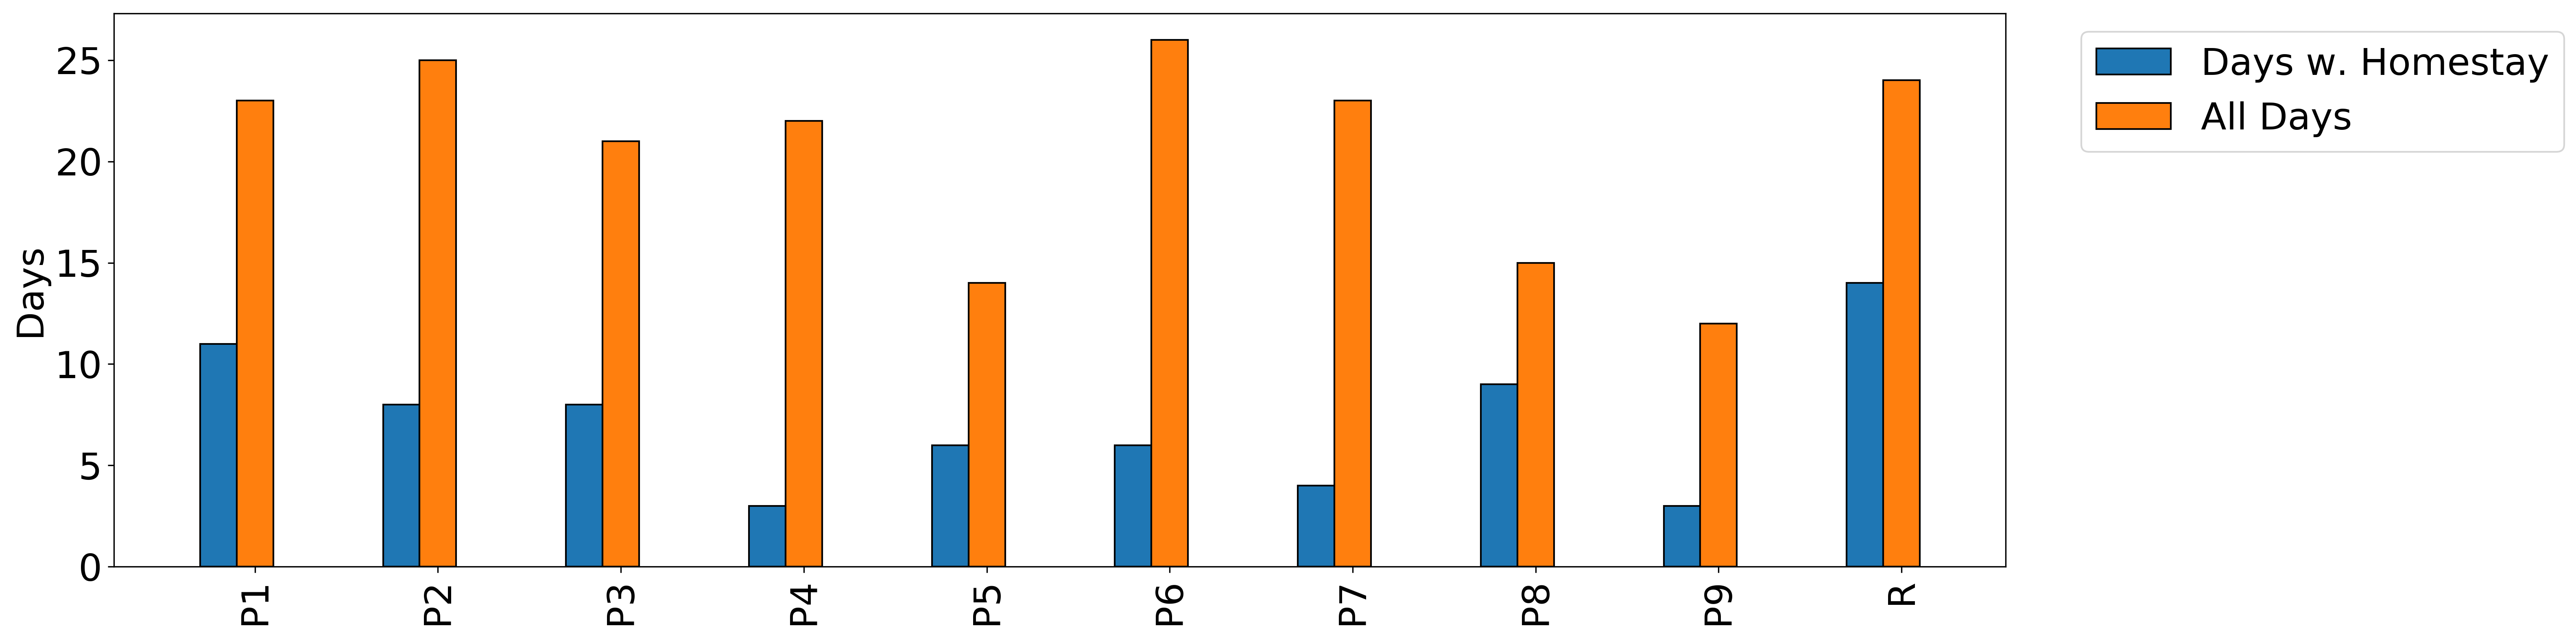
\includegraphics[width=\textwidth]{images/study/homestay_valid_days.png}
    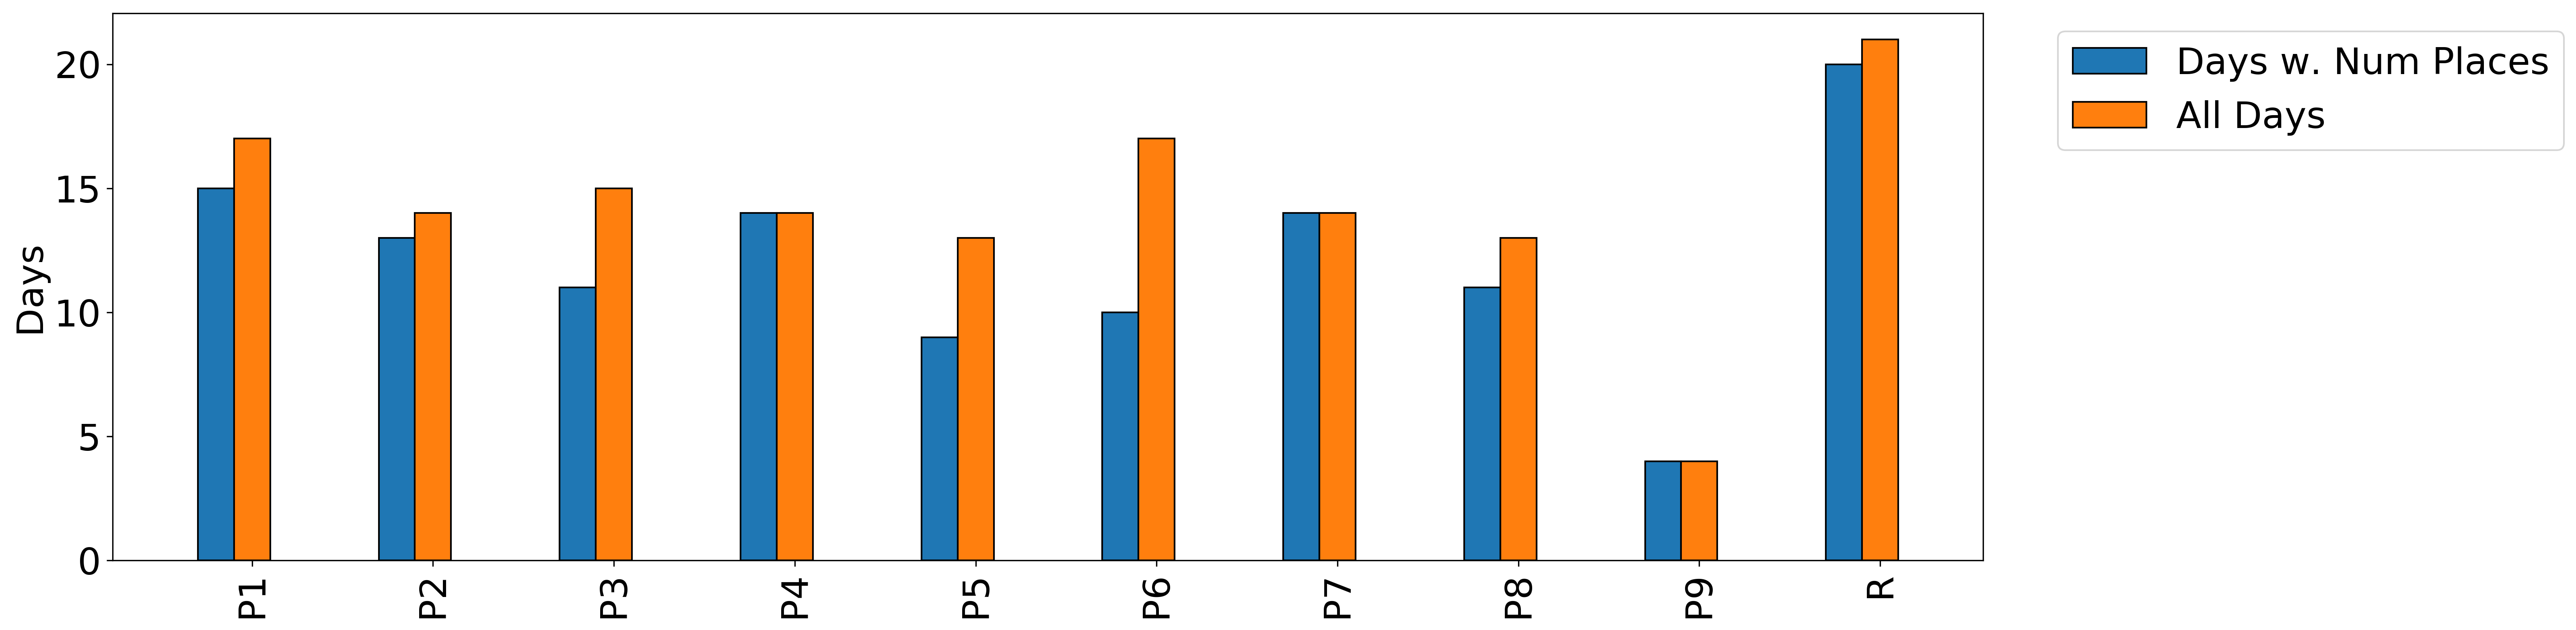
\includegraphics[width=\textwidth]{images/study/numplaces_valid_days.png}
    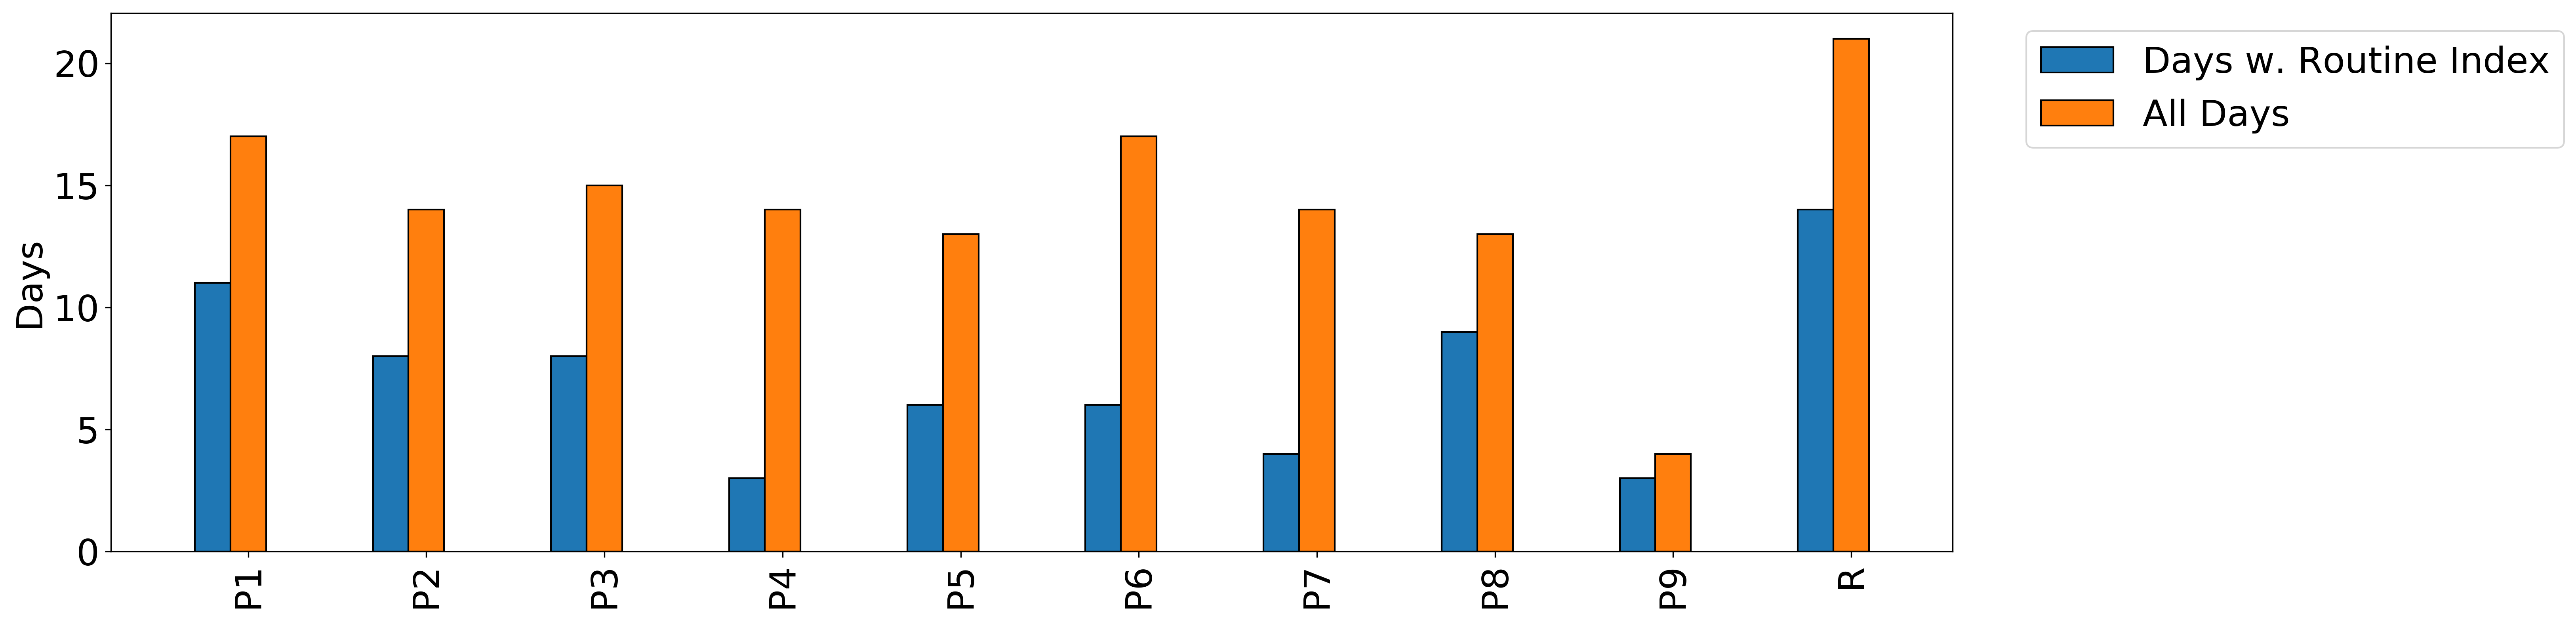
\includegraphics[width=\textwidth]{images/study/routine_valid_days.png}
    \caption{The days for which a given feature could be evaluated, out of the total days for which an answer was given and features were computed}
    \label{fig:plot-daily}
\end{figure}

Since the Home Stay feature is calculated by using the \textit{tracked} time at home, divided by the total time time midnight, it only takes a few minutes of missing data to make the home stay feature undershoot. It is therefore to be expected that this feature will lie somewhat lower than the answer given by the user, given the user did not round up excessively.


\begin{figure}
    \centering
    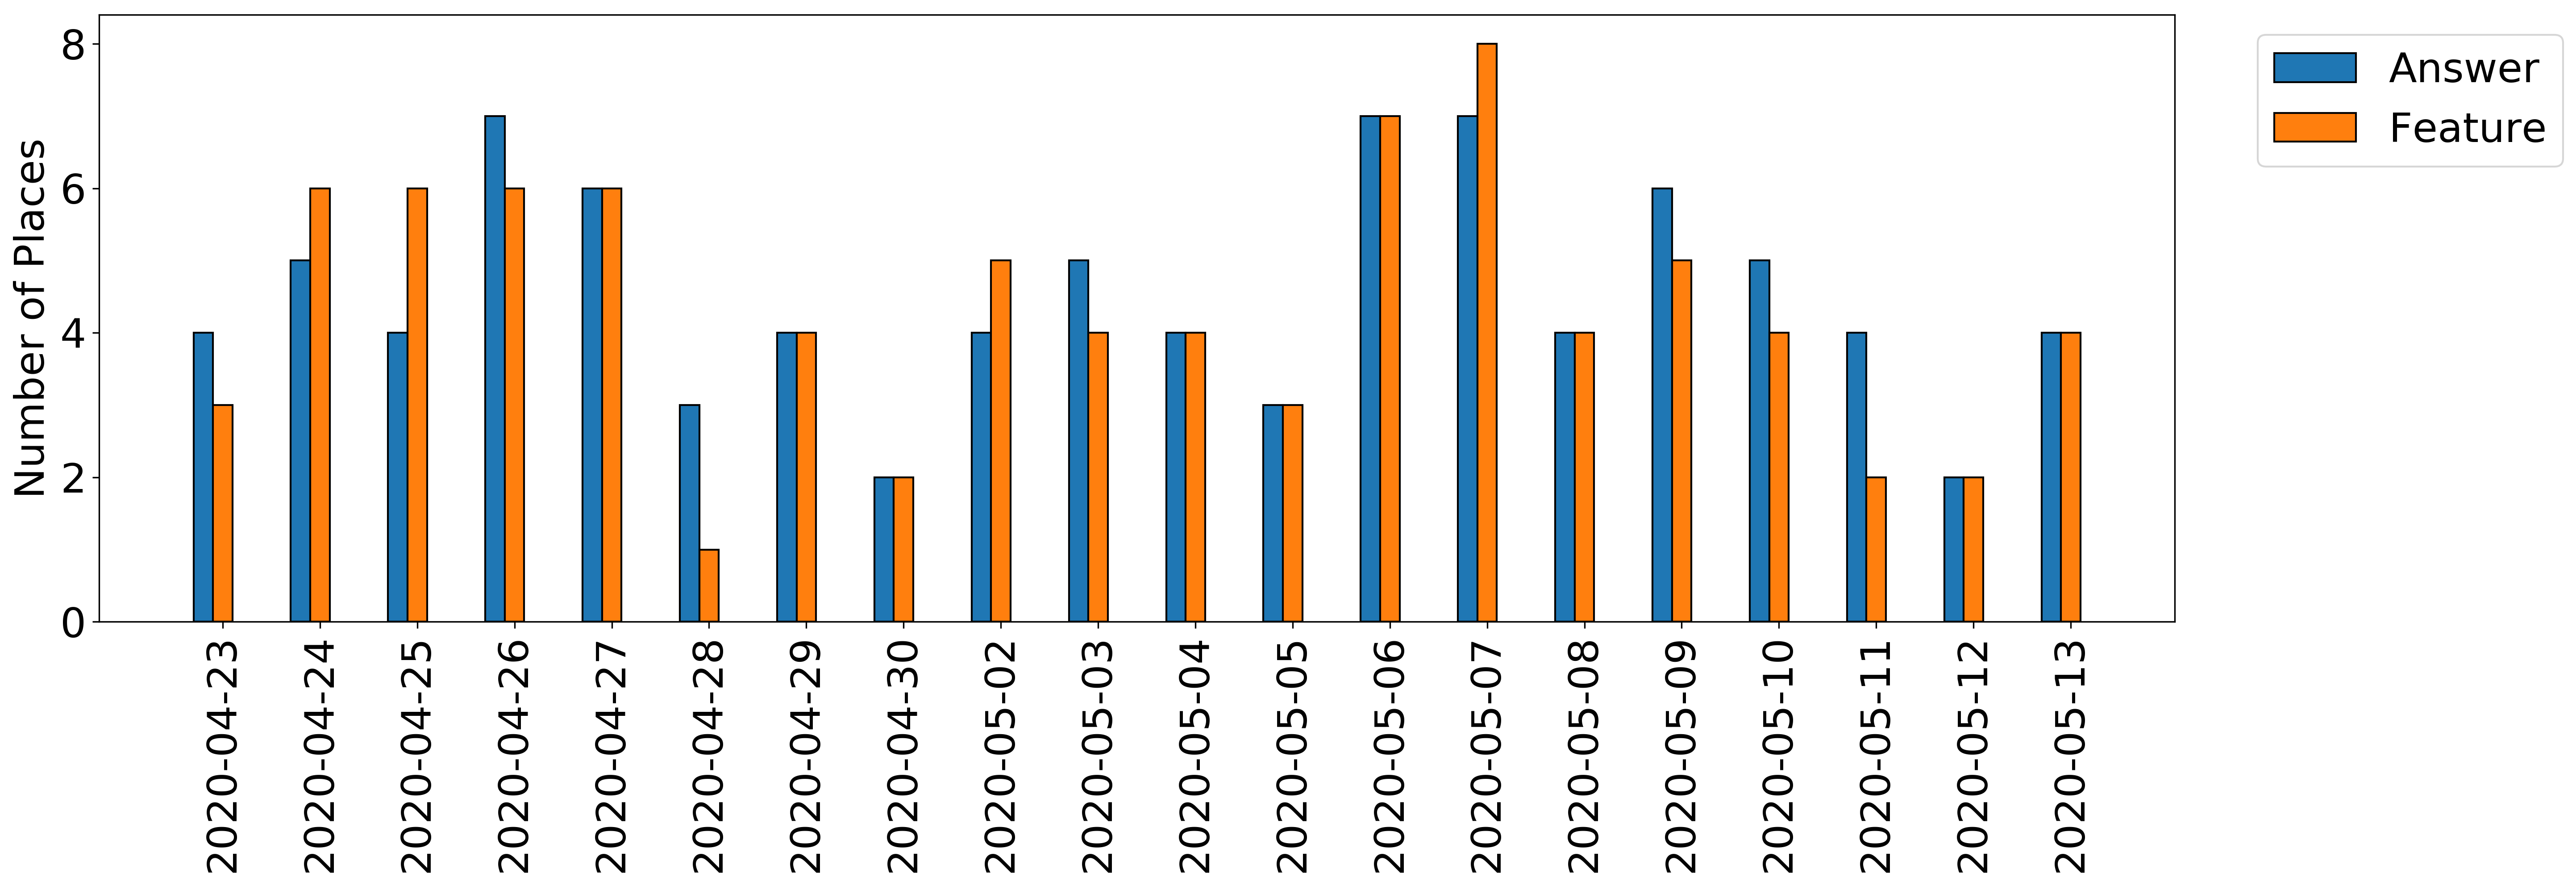
\includegraphics[width=\textwidth]{images/study/places_d6b2d9b9-398b-4e0d-b52b-224747f515c8.png}
    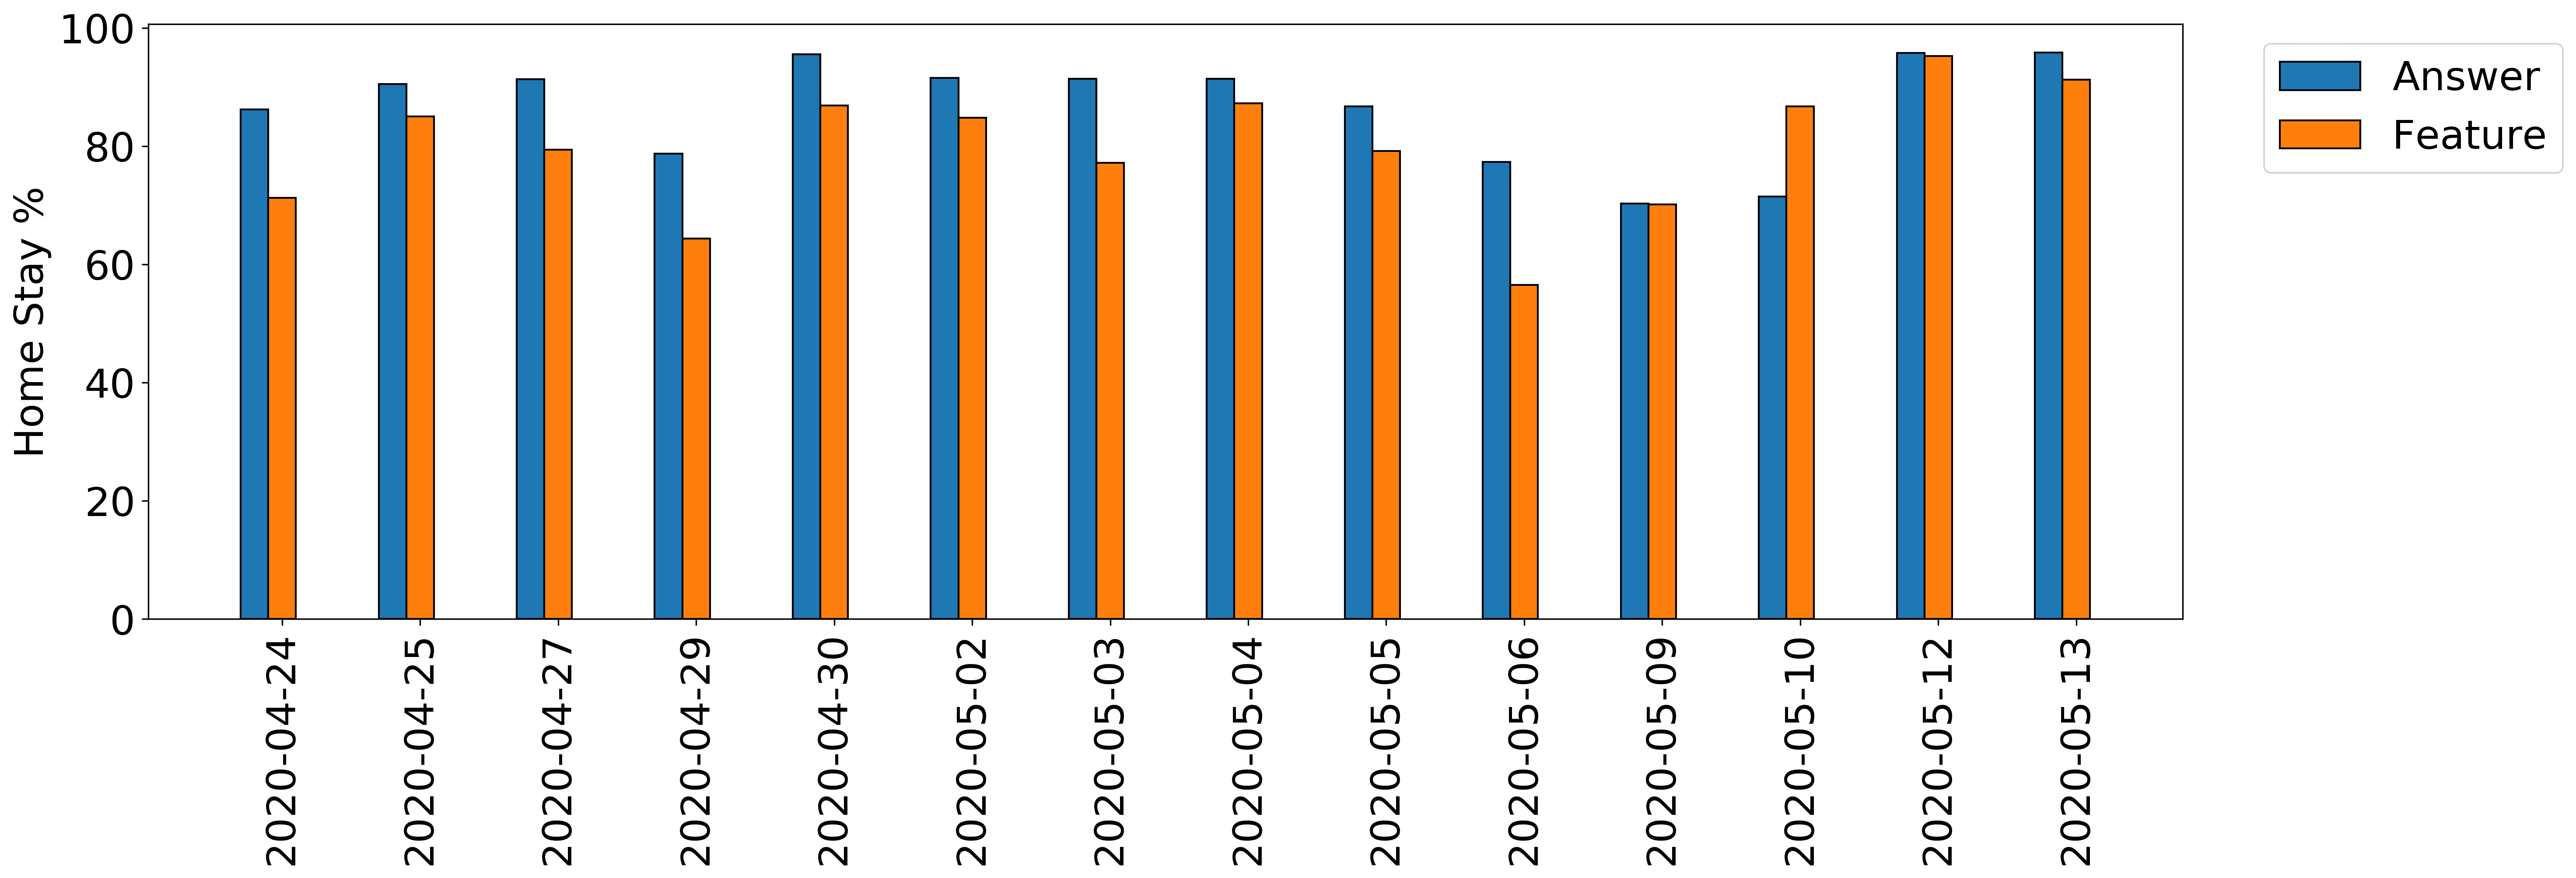
\includegraphics[width=\textwidth]{images/study/homestay_d6b2d9b9-398b-4e0d-b52b-224747f515c8.png}
    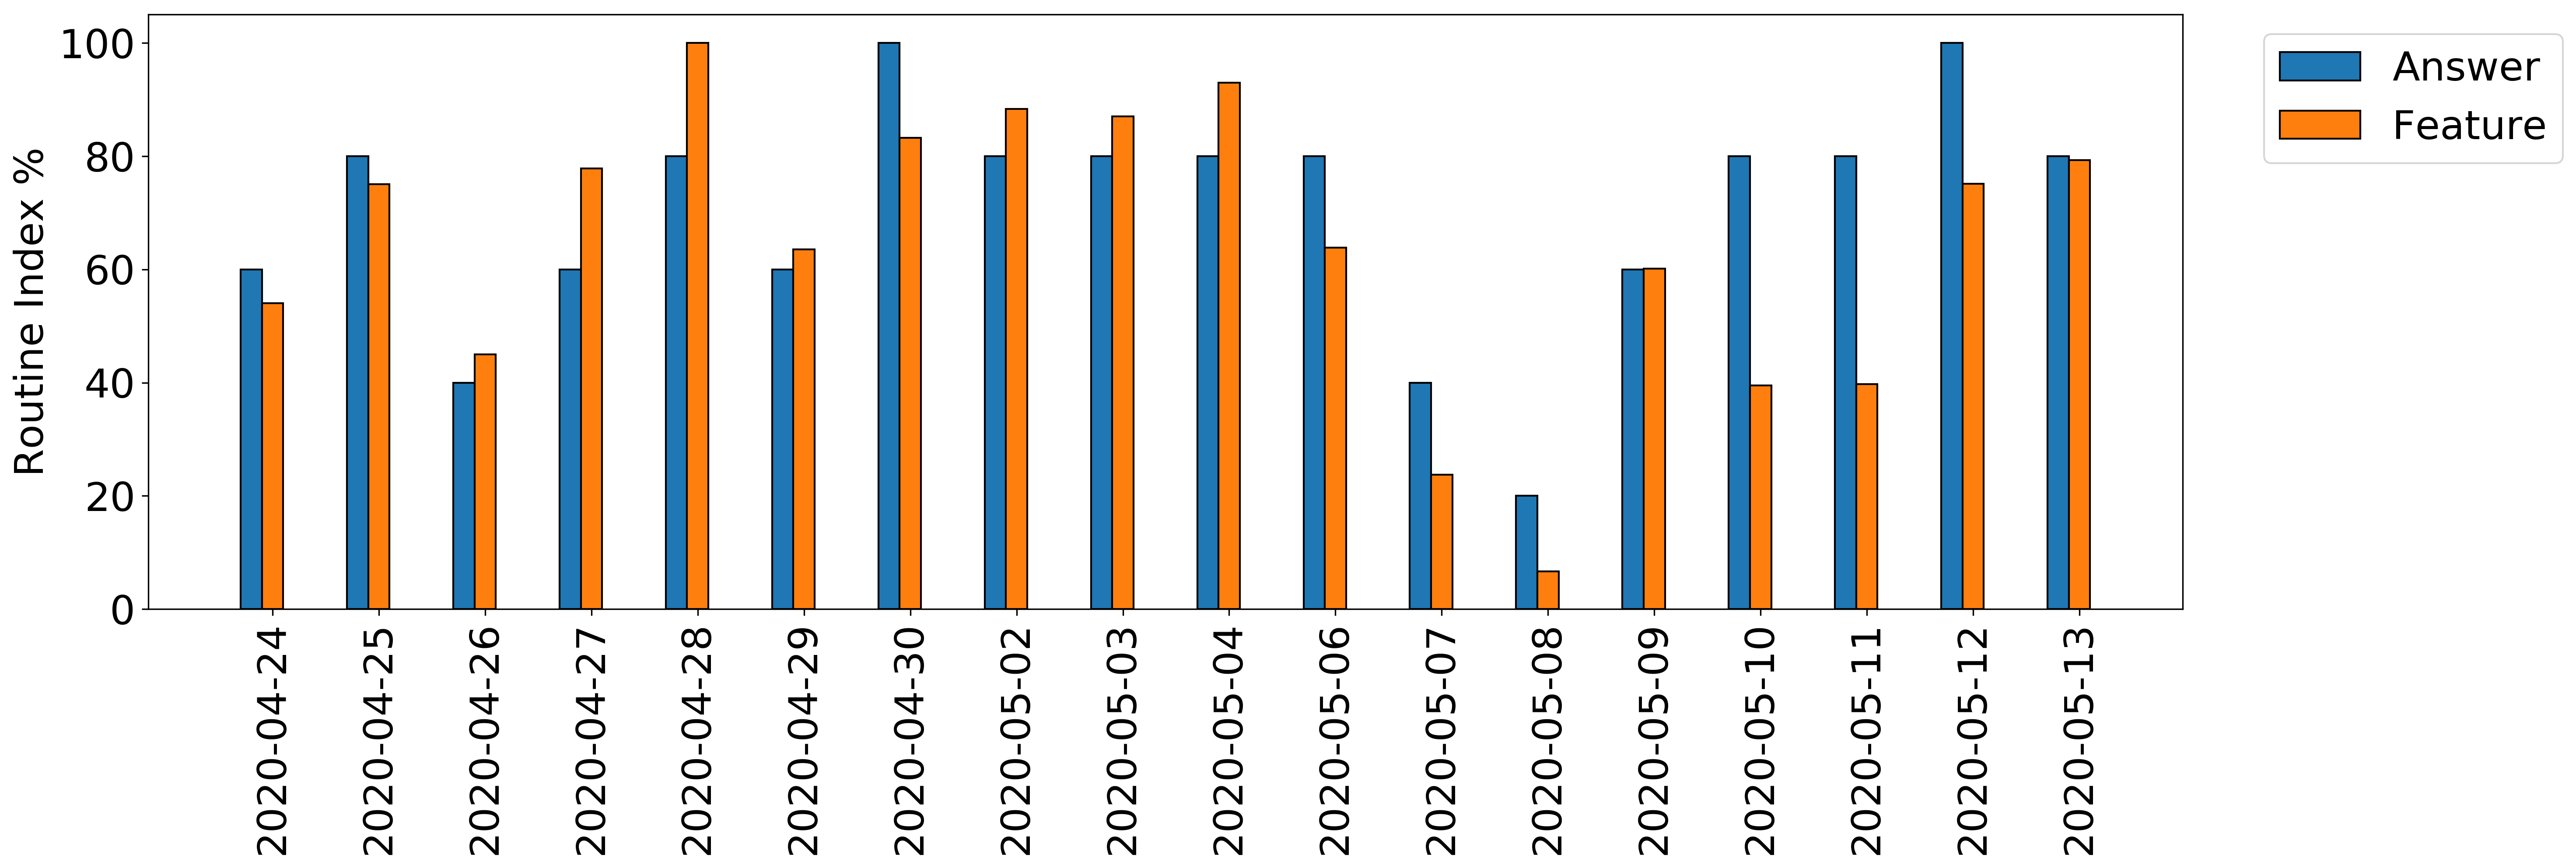
\includegraphics[width=\textwidth]{images/study/routine_d6b2d9b9-398b-4e0d-b52b-224747f515c8.png}
    \caption{The answered and calculated data for each day, for the author}
    \label{fig:plot-author-features}
\end{figure}

The day-by-day results for the author are displayed in figure \ref{fig:plot-daily} and from this plot the computed features have a high correspondence with the provided answers. However, the feature computation is based on the authors own definitions which means the computed features and answers of the author are also expected to be highly correlated. It is therefore relevant to show another participant, namely participant P8, who was very diligent in answering and tracking their location data. For this participant, very promising results were also produced which can be seen in Figure \ref{fig:plot-participant-features}.

\begin{figure}
    \centering
    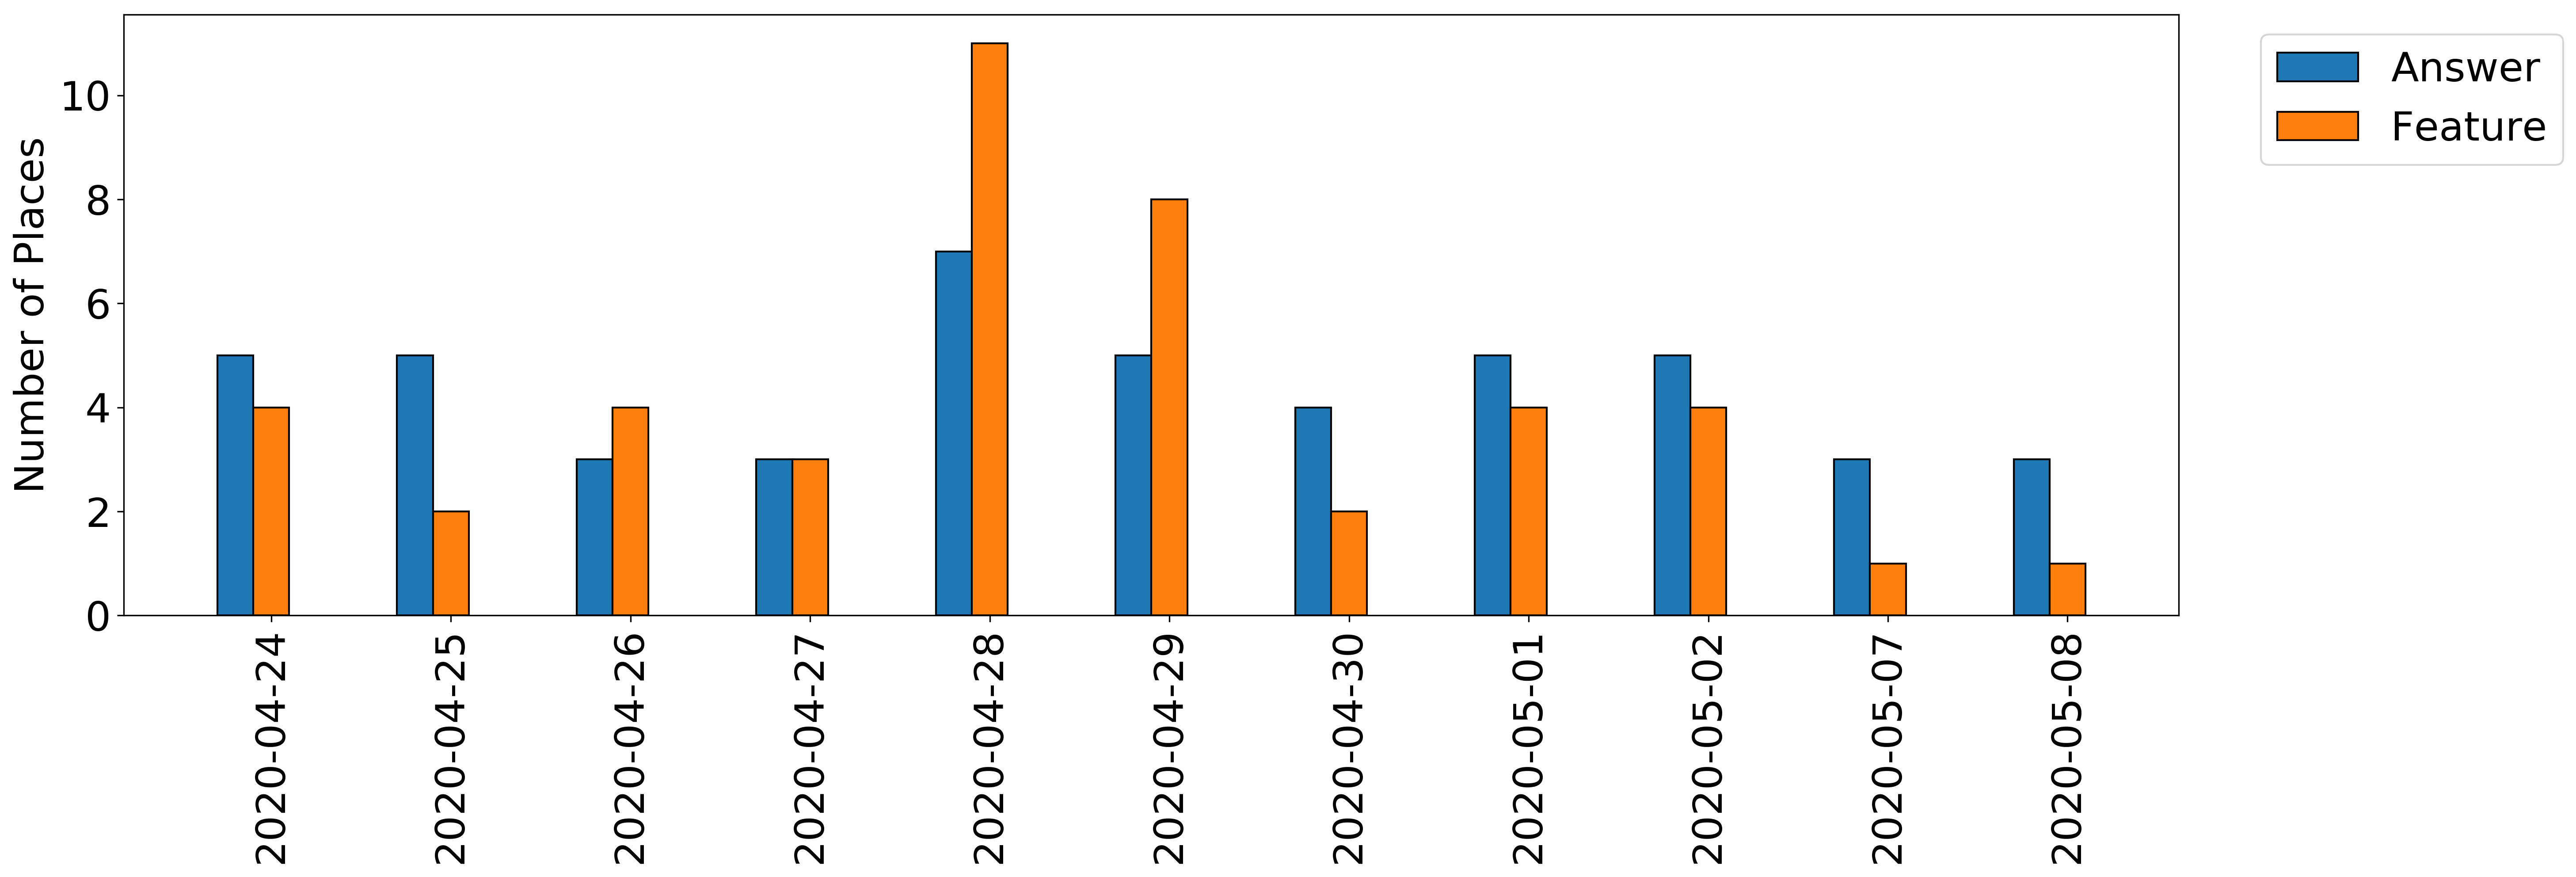
\includegraphics[width=\textwidth]{images/study/places_ec110976-0192-436d-b451-4f5dd97e71d8.png}
    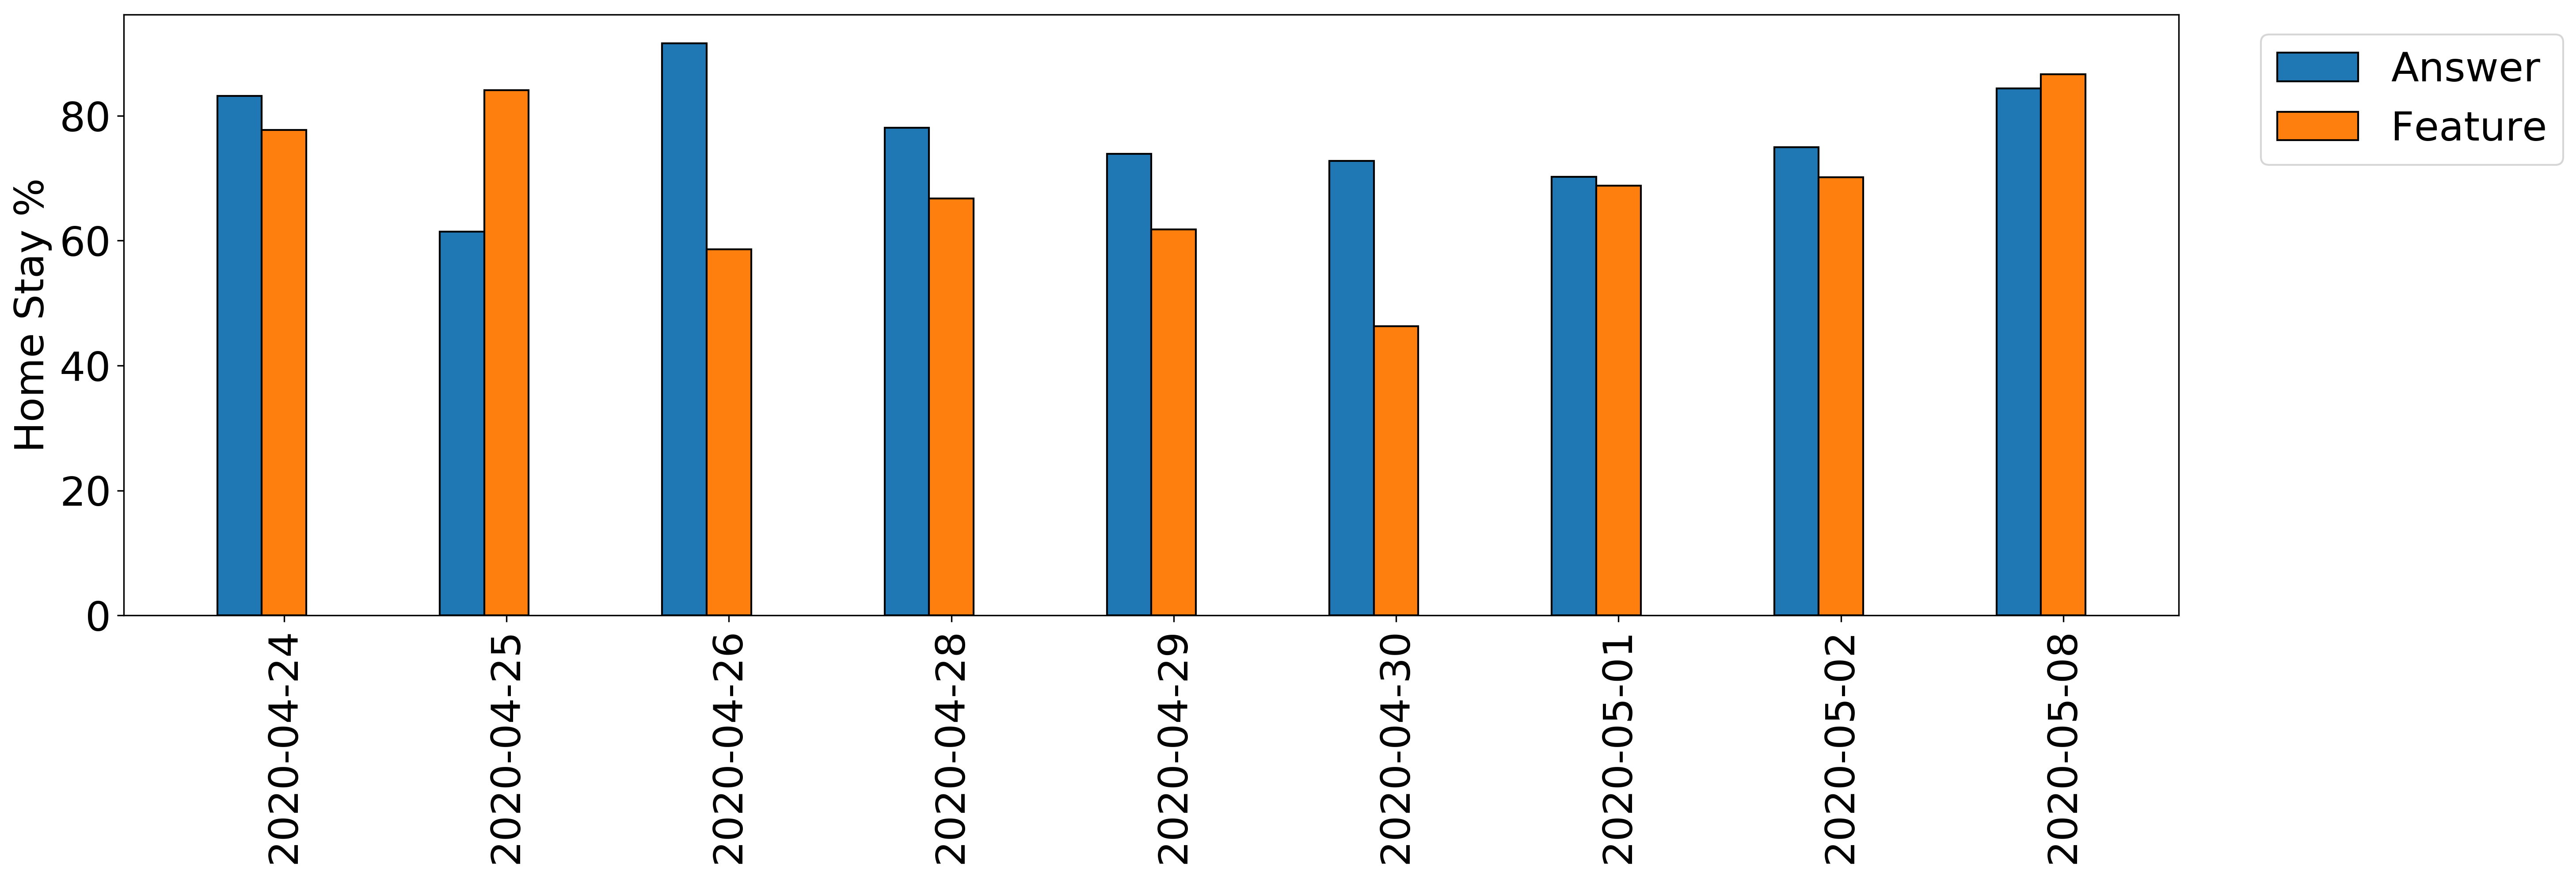
\includegraphics[width=\textwidth]{images/study/homestay_ec110976-0192-436d-b451-4f5dd97e71d8.png}
    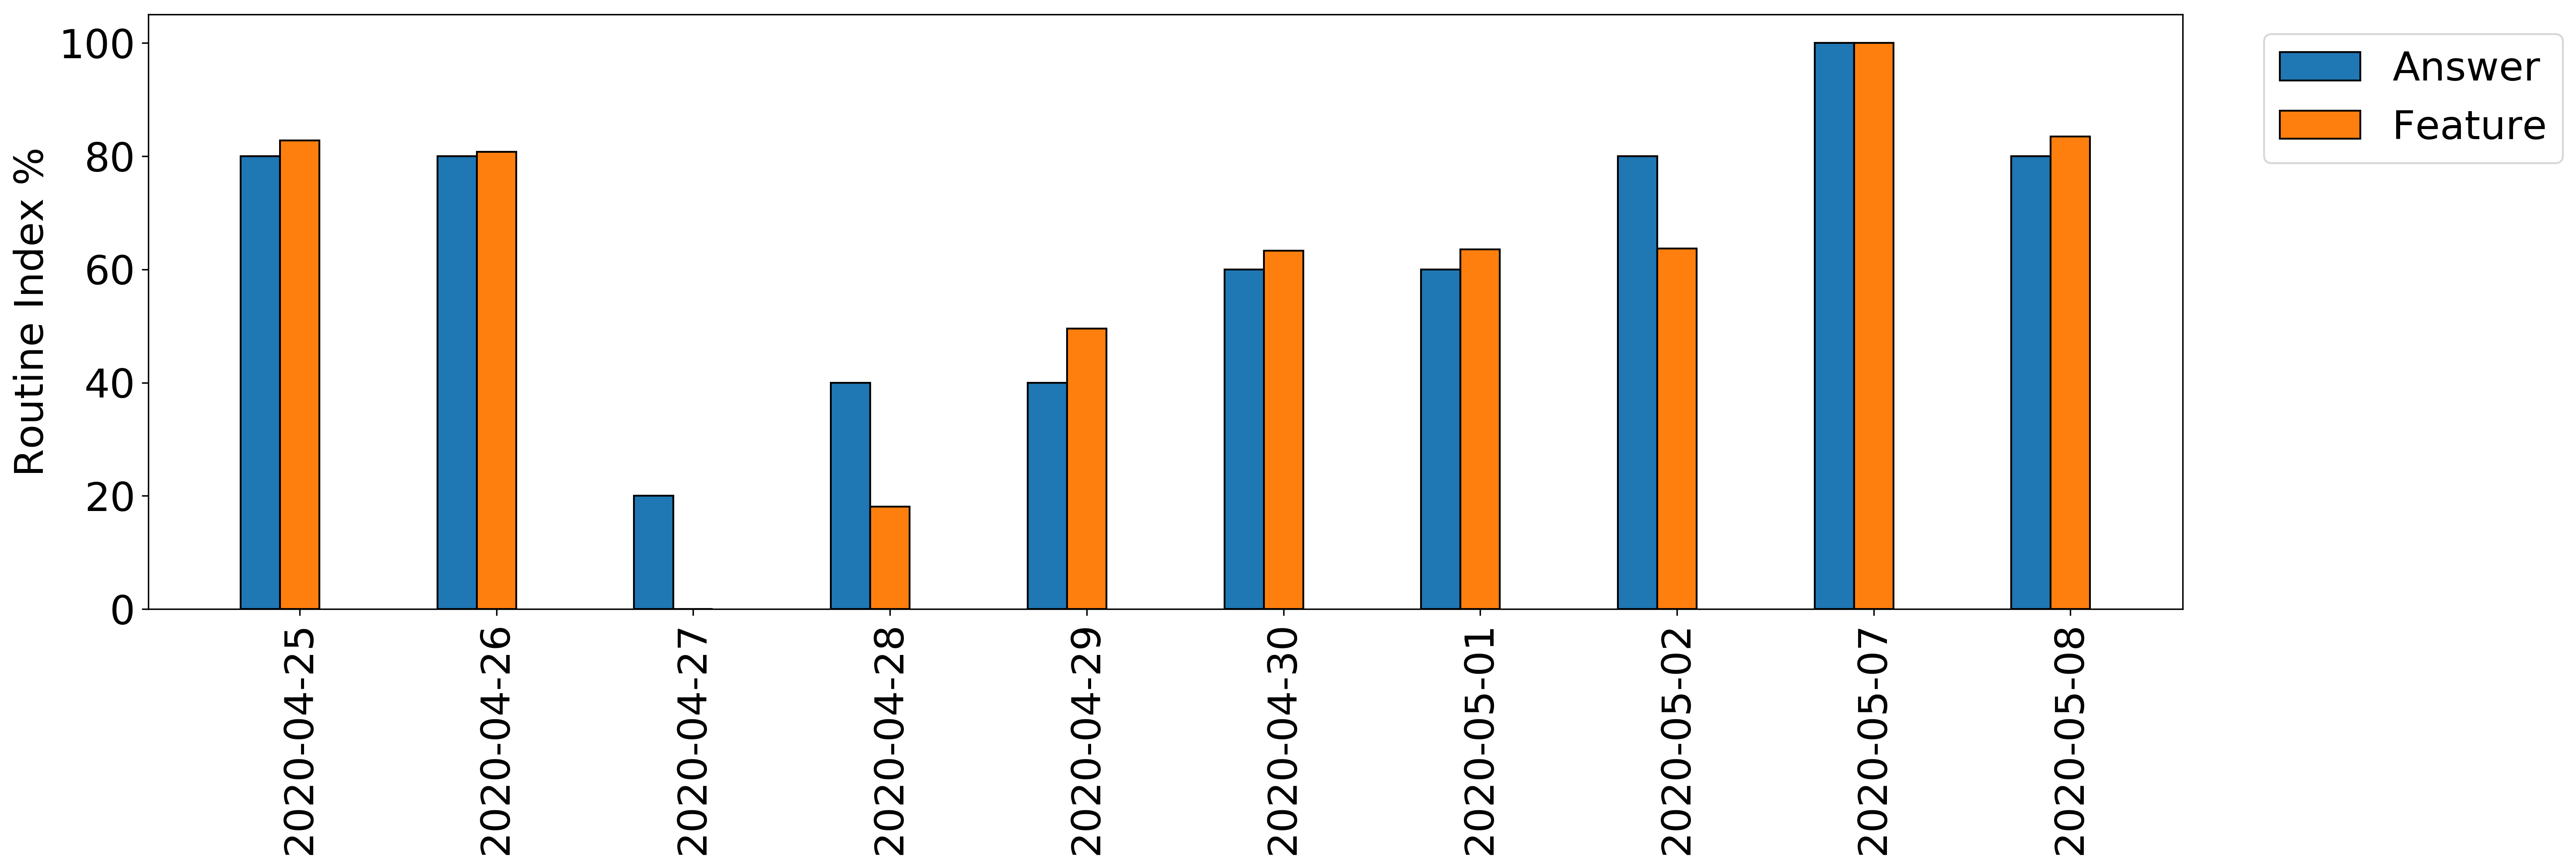
\includegraphics[width=\textwidth]{images/study/routine_ec110976-0192-436d-b451-4f5dd97e71d8.png}
    \caption{The answered and calculated data for each day for a participant P7}
    \label{fig:plot-participant-features}
\end{figure}
\subsection{Measuring Errors}

To say something about whether or not the algorithms undershoots or overshoots, the difference in sum was calculated as $ME = \frac{\sum(A) - \sum(F)}{N}$ ($N$ being the total number of days for the specific feature) meaning that if the result is positive then the answered result was on average higher and vice versa if the result is negative. The alternative is to calculate the mean error one can also calculate the mean of the difference per observation $ME = \frac{1}{N} \sum_{i=0}^{N} (a_i - f_i)$ however this the downside of cancelling out certain observations when the sign differs. Figure \ref{fig:plot-mean-error} shows the mean error for each feature, for each participant. It can be observed that participants generally answer that they have been at more places than the algorithms calculate. The Home Stay feature generally lies 10\% lower for half the participants (i.e. positive mean error), which was to be expected for reasons discussed earlier. For a couple of participants it overshoots (i.e. negative mean error) although still within 10\% error. For participant 2 however it averages out to near zero percent and for participant P1 the feature undershoots dramatically with an error of 30\%. The Routine Index feature is a mixed bag, with 6 participants answering higher than the algorithm and the remaining 4 being lower. All except for participant 6 deviating with almost 40\%. An important detail here is that the Routine Index answer was given on  scale with 20 percent increments which means that the mean error is likely to lie much higher percentage-wise than the other two features.

\begin{figure}
    \centering
    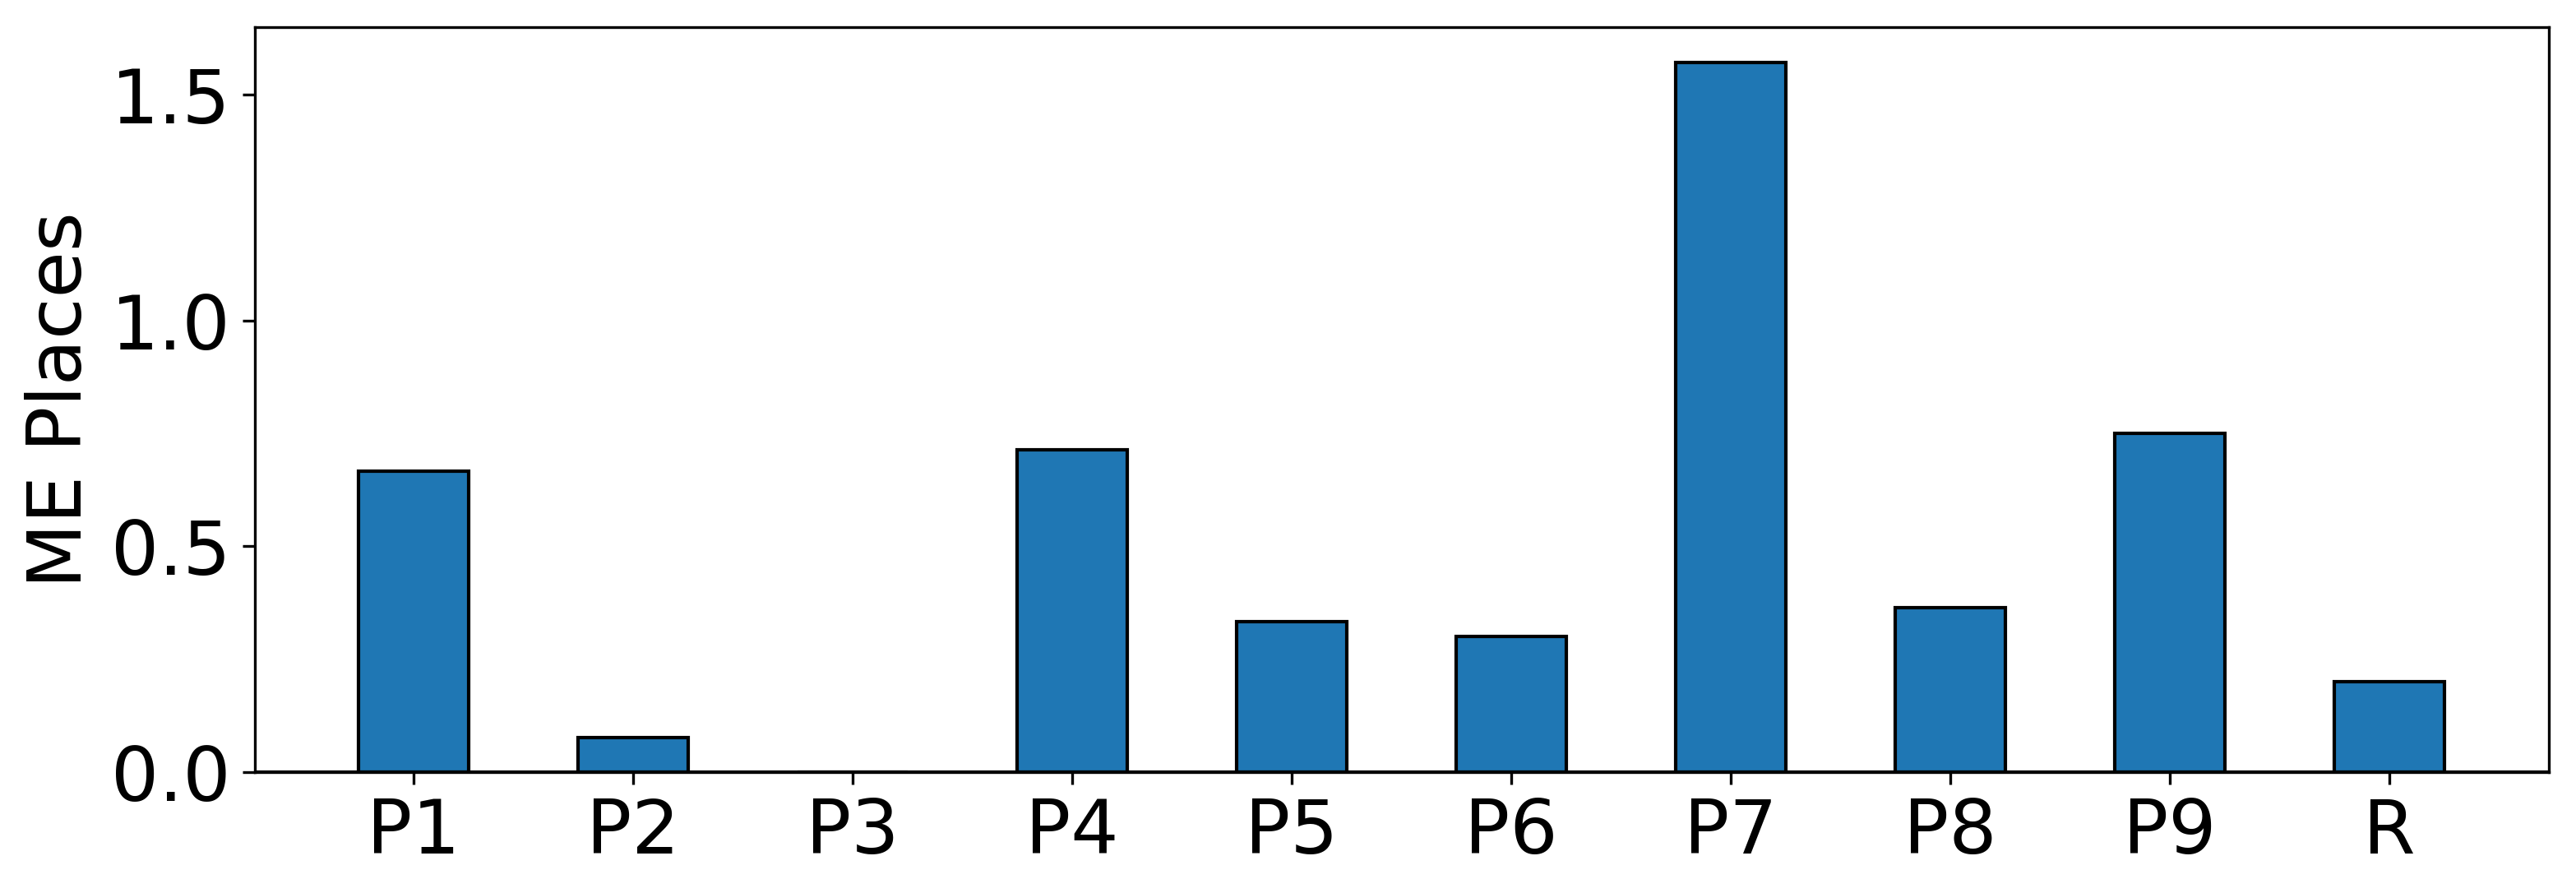
\includegraphics[width=\textwidth]{images/study/me_places.png}
    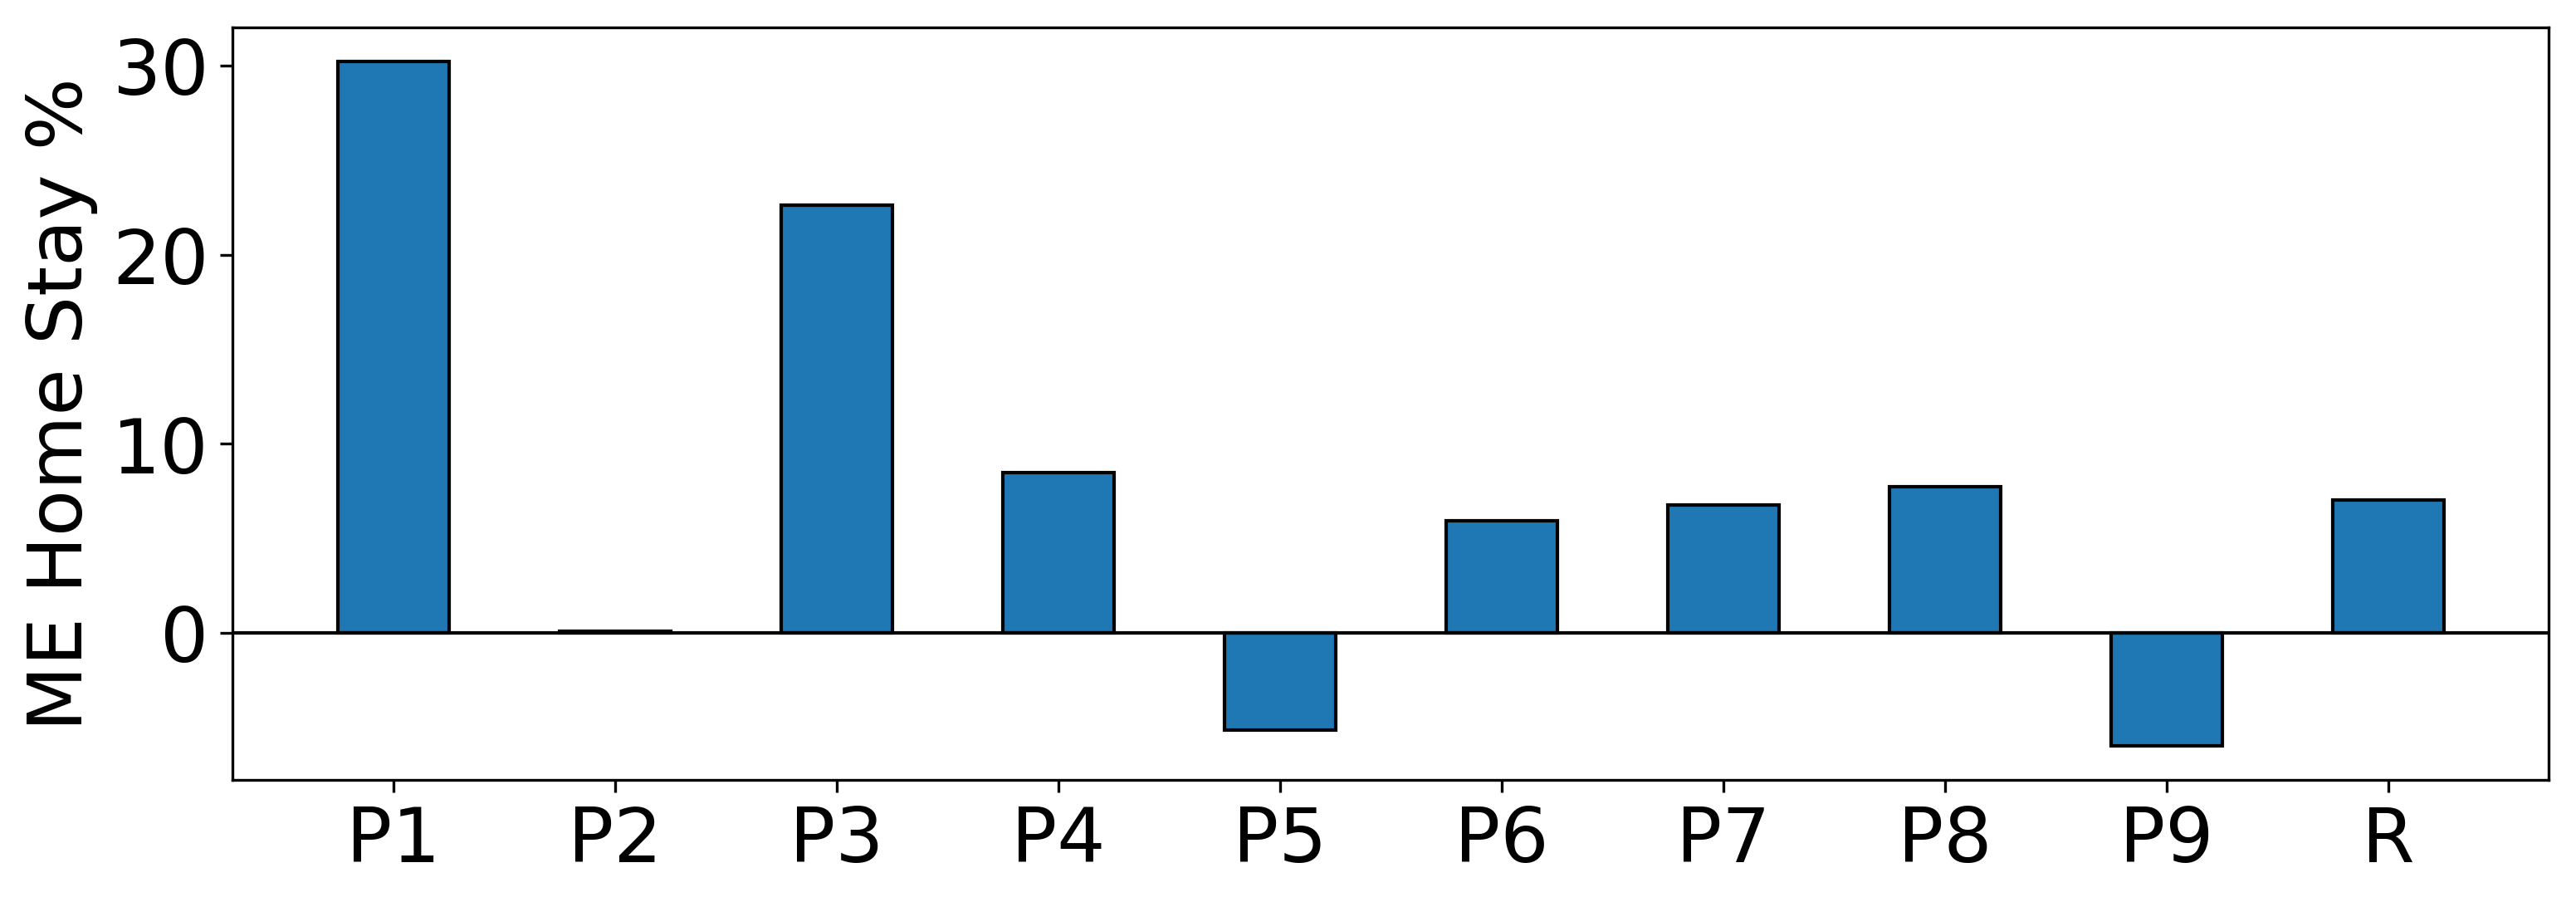
\includegraphics[width=\textwidth]{images/study/me_homestay.png}
    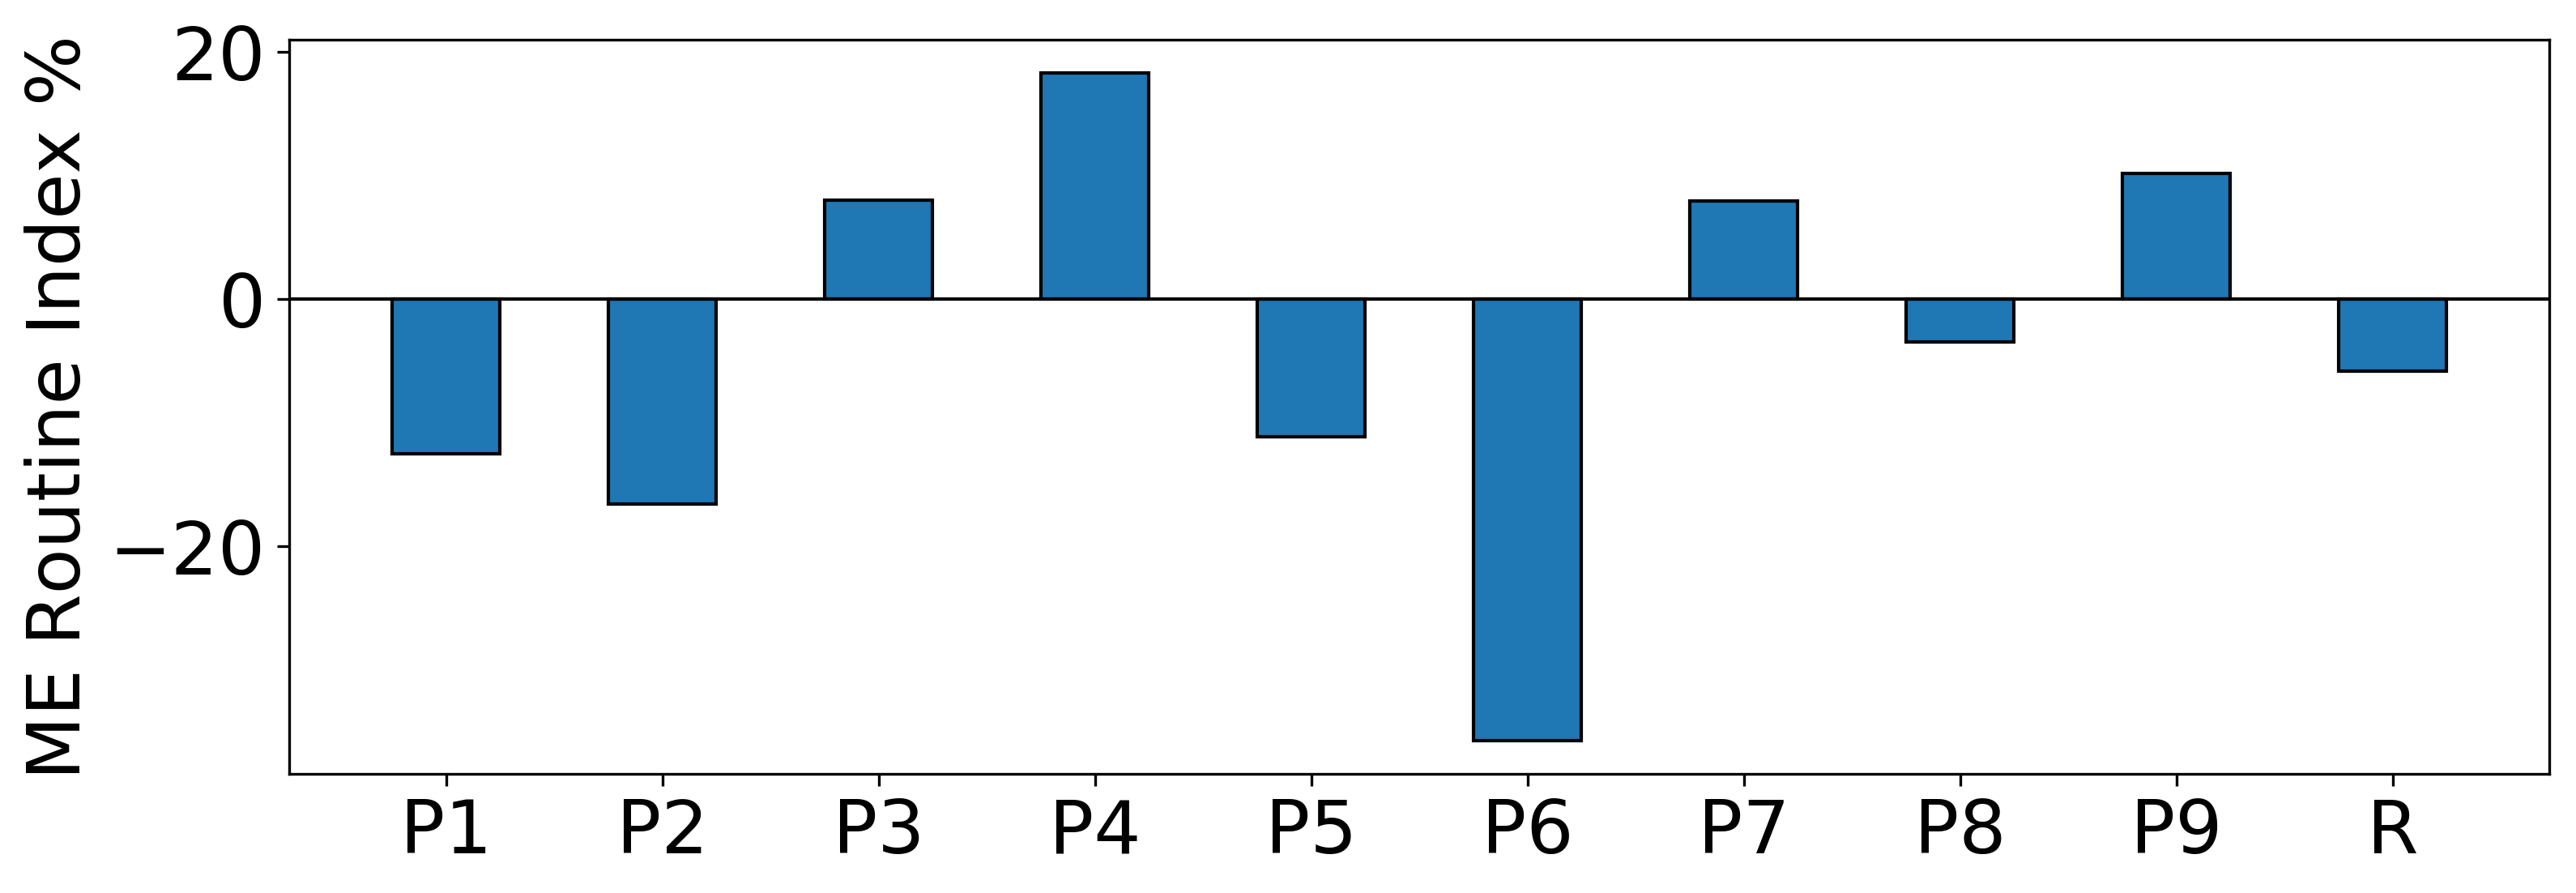
\includegraphics[width=\textwidth]{images/study/me_routine.png}
    \caption{The number of data points in terms of days which could be evaluated, for each participant}
    \label{fig:plot-mean-error}
\end{figure}


